\documentclass[12pt,oneside]{memoir}

\usepackage{nus-bcomp-fyp}

\addbibresource{references.bib}

\title{Benchmarking and Improving OCR Systems for Southeast Asian Languages}
\author{Qiu Jiasheng, Jason}
\department{Department of Computer Science}
\faculty{School of Computing}
\university{National University of Singapore}
\academicyear{2024/2025}
\projectid{H0792230}
\supervisor{A/P Min-Yen Kan}
\advisor{Tongyao Zhu}

\begin{document}
\frontmatter

\pagestyle{plain}

\makecover

\setcounter{page}{1}

\maketitle
\addcontentsline{toc}{chapter}{Title}

\chapter*{\centering\large Abstract}
\addcontentsline{toc}{chapter}{Abstract}

While Optical Character Recognition (OCR) has been widely studied for high-resource languages such as English and Chinese, the efficacy and limitations of OCR models on Southeast Asian (SEA) languages remain largely unexplored. This study aims to bridge this gap by evaluating OCR technologies for SEA languages and exploring script-specific challenges. We propose a pipeline to collect textual data from Wikipedia and benchmark open-source OCR tools. Additionally, we demonstrate the potential of fine-tuning existing models on SEA languages, aiming to expand OCR capabilities for these languages.

\vspace{20pt}
Subject Descriptors:

\hspace*{0.3in} H.3.3 Information Search and Retrieval

\hspace*{0.3in} I.2.7 Natural Language Processing

\hspace*{0.3in} I.2.10 Vision and Scene Understanding

Keywords:

\hspace*{0.3in} Optical Character Recognition, Southeast Asian Languages, Fine-tuning

Implementation Software and Hardware:

\hspace*{0.3in} Python, Tesseract, EasyOCR, General OCR Theory

\chapter*{\centering\large Acknowledgements}
\addcontentsline{toc}{chapter}{Acknowledgements}

I would like to express my deepest appreciation to my supervisor, A/P Kan Min-Yen, and my advisor, Tongyao Zhu, for their invaluable guidance and suggestions in every step of my research. 
Their encouragement and constructive feedback have been a significant source of inspiration throughout the past year.
I am grateful for their constant patience and support in guiding me to complete the project.

I would also like to thank the members of the Web, Information Retrieval / Natural Language Processing Group (WING) for listening to my practice presentations and offering valuable feedback. 
I am thankful for the opportunity to attend the group meetings and hear about the group's amazing work in the academic field.

Finally, I would like to thank my family and friends for their unwavering support and confidence in me.
Even though they did not understand the technical aspects of my project (the number of times I had to explain OCR in the past year is insane), their constant care for my progress and well-being deeply encouraged me.

\listoffigures
\listoftables
\tableofcontents

\mainmatter

\chapter{Introduction}
Current research in Natural Language Processing (NLP) is heavily concentrated on only 20 of the 7,000 languages in the world \parencite{magueresse-etal-2020}.
In particular, Southeast Asia (SEA) is home to over 1,000 languages but remains a relatively under-researched region in NLP \parencite{aji-etal-2023}.
A similar trend can be observed in Optical Character Recognition (OCR) research, where the focus is predominantly on high-resource languages \parencite{salehudin-etal-2023, smith-2007}, leaving many SEA languages underserved.

OCR, the process of converting textual images into machine-readable formats, offers significant potential for languages with limited datasets. While many scanned documents and books in these low-resource languages are available online, the text within them often remains inaccessible due to formats like images and PDFs. By extracting the text from these documents, OCR can generate valuable datasets for low-resource languages, which can then be used for downstream NLP tasks, such as machine translation and named entity recognition \parencite{agarwal-and-anastasopoulos-2024, ignat-etal-2022}.
Therefore, studying OCR performance on SEA languages is crucial to accelerating NLP research and technology development in the region.

While OCR has been widely studied for high-resource languages such as English and Chinese, the efficacy and limitations of OCR models on SEA languages remain largely unexplored.
To address this gap, this study aims to evaluate and enhance the performance of OCR technologies on SEA languages, thereby advancing NLP applications in this linguistically diverse region.
Specifically, this project seeks to answer the following research questions (RQs):

\begin{itemize}
    \item \textbf{RQ1:} How do popular OCR tools perform on SEA scripts?
    \item \textbf{RQ2:} What script-related challenges affect OCR accuracy on SEA languages?
    \item \textbf{RQ3:} How can fine-tuning enhance OCR accuracy on SEA languages?
\end{itemize}

To investigate these questions, we present a reusable pipeline for collecting textual data from Wikipedia and benchmarking three open-source OCR tools on English, Indonesian, Vietnamese, and Thai.
The source code of the pipeline is publicly available on \href{https://github.com/jasonqiu212/ocr-benchmarking-on-sea-languages}{GitHub}.

Our benchmark results reveal that OCR tools generally perform worse on Vietnamese and Thai texts.
However, contrary to common assumptions, they perform well on the native characters of these languages. 
This challenges the prevalent notion that Latin-based scripts inherently yield better OCR performance than more complex scripts such as Vietnamese and Thai.
Instead, we find that the main source of errors stems from the misclassification of characters outside the target language, highlighting the need for OCR systems to better handle mixed-script content for higher accuracy.

Furthermore, we demonstrate the potential of fine-tuning a transformer-based model to improve OCR performance on Vietnamese and Thai. 
The fine-tuned model achieved error rates of 0.10 for Vietnamese and 0.15 for Thai, representing a significant improvement over the base model.
These results underscore fine-tuning as an effective strategy for adapting OCR systems to new languages.

\chapter{Related Work}

\section{Overview of OCR Systems}

Most OCR systems consist of two stages: text detection and text transcription.
Text detection identifies text present in an image and extracts cropped regions containing the detected text. 
A text transcription model then converts these cropped images into text.
Generally, separate models are used for each stage, allowing for greater training flexibility and a clearer understanding of challenges within each component \parencite{subramani-etal-2023}. 
More recently, end-to-end models that combine both stages have shown promise in reducing errors for certain use cases \parencite{feng-etal-2019}.

\subsection{Evolution of OCR Models}

Early OCR models employ traditional machine learning techniques, such as K-nearest Neighbors (KNN) and Support Vector Machines (SVMs), to classify textual characters from cropped images \parencite{ghadekar-etal-2018}.
Tesseract, an established OCR engine developed since the 1990s, recognizes character patterns by extracting small fragments of character outlines as features \parencite{smith-2013}.
These features are then classified into character clusters using an optimized KNN algorithm.

The rise of deep learning brought significant advancements in OCR.
Convolutional Neural Networks (CNNs) improve feature extraction by automatically detecting edges, textures, and shapes within text images.
Unlike traditional handcrafted features, CNNs learn visual patterns by applying small filters across an image. 
The Character Region Awareness for Text Detection (CRAFT) algorithm, for example, uses a fully convolutional network to achieve state-of-the-art character localization \parencite{baek-etal-2019}.
For text transcription, Recurrent Neural Networks (RNNs) have been widely adopted due to their ability to model sequential dependencies over time.
Tesseract 4.0 integrated a Long Short-Term Memory (LSTM) model, a specialized type of RNN, to recognize entire lines of text instead of individual characters \parencite{tesseract-2025}.
By combining CNNs for feature extraction and RNNs for sequence modeling, \textcite{shi-etal-2015} proposed the Convolutional Recurrent Neural Network (CRNN), which significantly improved text recognition accuracy in end-to-end OCR systems.

More recently, transformer-based models have emerged as a powerful alternative.
Unlike CNNs and RNNs, transformers process entire input sequences in parallel using self-attention mechanisms, which allows them to capture long-range dependencies in text images more efficiently \parencite{vaswani-2017}.
This approach avoids image-specific inductive biases present in CNNs, such as the assumption that neighboring pixels are relevant.
TrOCR, an end-to-end model that combines an image transformer and a separate text transformer, demonstrates another advantage of transformers: the ability to leverage self-supervised pre-training \parencite{li-etal-2021}. 
Since transformers can be pre-trained individually to learn useful patterns from unlabeled images and text, there is less reliance on manually annotated OCR training data to achieve high accuracy.
Going beyond traditional text recognition, General OCR Theory (GOT) is another transformer-based model that extends character recognition capabilities to non-text elements, such as sheet music, charts, and geometric shapes \parencite{wei-etal-2024}.
By integrating Large Visual-Language Models (LVLMs), GOT seeks to address the bottlenecks of traditional OCR systems, which often struggle with generalization.
As transformer-based OCR continues to evolve, these models are expected to push the boundaries of text recognition, enabling more flexible and adaptable OCR systems for diverse applications.

While deep learning techniques for OCR have been widely studied, there is still limited research focused on the performance of transformer-based OCR models, particularly for SEA languages.
Our research compares the performance of various OCR tools, including those using transformer-based architectures, on SEA languages. 
In doing so, we aim to explore how these models handle text recognition in more complex and diverse linguistic contexts.

\section{Benchmarking OCR on Low-resource Languages}

To evaluate OCR performance accurately, textual data in the form of images or PDFs paired with reliable ground truth is essential. 
Similar to most NLP tasks, data scarcity poses a major obstacle to advancing OCR technology in low-resource languages. The limited availability of annotated textual data restricts both model training and evaluation, leading to disparities in OCR accuracy across different scripts.
OCR tools generally perform better on Latin-based scripts \parencite{hegghammer-2022}, partly due to market incentives that prioritize the development of English-language OCR systems, resulting in more extensive training data and refinement.
Beyond data availability, the complexity of scripts with ornate diacritics or unique letter shapes often yields lower OCR accuracy \parencite{agarwal-and-anastasopoulos-2024}.

A recent study by \textcite{ignat-etal-2022} provides the most relevant benchmarking of OCR on SEA languages.
Their benchmark grouped 60 low-resource languages by region and script, including SEA languages such as Khmer, Lao, Burmese, Thai, and Vietnamese.
They found that OCR tools perform best on Latin and Cyrillic scripts, with only average performance on SEA languages, supporting \textcite{hegghammer-2022}'s findings.
Additionally, \textcite{ignat-etal-2022} showed that while OCR models perform well on synthetic SEA language data, their accuracy drops significantly on real-world data.
This discrepancy underscores the need for more diverse and realistic training datasets to improve OCR outcomes for SEA languages.
Our research aims to address this gap by developing a reusable pipeline for both collecting real-world digital data and generating synthetic data.

\section{Using Synthetic Data for OCR Evaluation}

To bridge the gap in data availability, many studies rely on artificial images and PDFs generated from plain text to create evaluation datasets.
For instance, \textcite{ignat-etal-2022} generated synthetic PDFs from the Flores 101 dataset, which consists of text from Wikipedia in 101 languages.
Expanding on this approach, \textcite{gupte-etal-2021} developed an open-source Python package that creates document images from plain text, incorporating several document styling templates.
These methods enable the large-scale generation of high-quality, low-resource language data with corresponding ground truth annotations.

However, one challenge with artificial datasets is their tendency to lack the imperfections found in real-world documents. 
Real-world scanned documents often feature complex layouts, stains, and handwritten scribbles \parencite{hegghammer-2022}. 
Studies have shown that OCR systems often perform better on synthetic datasets than on real-world data, highlighting a gap in generalization \parencite{ignat-etal-2022}.
To address this, researchers frequently apply noise augmentation to synthetic documents. 
Common techniques include changing the font style, size, color, and letter spacing, as well as adding Gaussian blur, bleed-through effects, and salt-and-pepper noise \parencite{gupte-etal-2021, ignat-etal-2022}.
These modifications help artificial datasets to better approximate the challenges of real-world OCR tasks.
Our study adopts similar techniques by generating and benchmarking on synthetic data with noise, aiming to better simulate the imperfections found in real-world documents.

\section{Fine-tuning OCR Systems}

To enhance OCR performance in new domains with limited labeled data, many studies explore fine-tuning, or further training pre-trained models on a smaller, task-specific dataset. 
Instead of training from scratch, fine-tuning updates a model's existing weights, allowing it to adapt to new datasets while retaining prior knowledge. 
For instance, \textcite{parres-and-paredes-2023} demonstrated that transformer-based models can successfully adapt to new languages and historical documents with minimal training data, achieving competitive OCR performance.
Similarly, \textcite{laurent-and-lauar-2024} fine-tuned the English TrOCR model for Spanish text, yielding strong results.
Fine-tuning thus offers a promising strategy for our research to overcome the scarcity of labeled data in low-resource languages while achieving high accuracy.

\chapter{Methodology}

To answer the research questions, this study conducted the following three experiments to benchmark and improve OCR performance on SEA languages:

\begin{itemize}
    \item \textbf{Experiment 1:} Benchmarking on Real-world Wikipedia Screenshots
    \item \textbf{Experiment 2:} Benchmarking on Synthetic Data
    \item \textbf{Experiment 3:} Fine-tuning for Vietnamese and Thai
\end{itemize}

\section{Experiment Setup}

\subsection{Languages}

In this study, we chose to benchmark on English, Indonesian, Vietnamese, and Thai. English serves as a baseline comparison due to its extensive OCR research and established tool support. Meanwhile, Indonesian, Vietnamese, and Thai were selected as a representative subset of SEA languages for several reasons.

Firstly, these three languages encompass a range of script types: Latin scripts for Indonesian, Latin scripts with diacritics for Vietnamese, and Brahmic scripts for Thai. 
By covering these scripts, we capture a broad spectrum of orthographic features, such as diacritics, tone marks, and complex character shapes. This allows us to examine how these unique linguistic features impact OCR performance. 
Furthermore, many other SEA languages, including Malay, Filipino, and Cebuano, use modified Latin scripts, while languages like Khmer, Burmese, and Javanese use Brahmic scripts. Thus, findings from this study can be applied to other languages with similar script types, accelerating OCR research in the region.

\begin{table}[ht]
    \centering
    \caption{Benchmarked Languages}
    \label{table:languages}
    \begin{tabular}{llll}
        \toprule
        & Speaker Population & Script Type & Example\\ 
        \midrule
        English & 1.5 billion & Latin & Good morning\\
        Indonesian & 252 million & Latin & Selamat pagi\\
        Vietnamese & 97 million & Latin with diacritics & Chào buổi sáng\\
        Thai & 71 million & Brahmic & {\fontspec{Tahoma} สวัสดีตอนเช้า}\\
        \bottomrule
        \multicolumn{4}{c}{\footnotesize Note: Speaker population data from Wikipedia (\citeyear{list-of-languages-by-total-number-of-speakers-2025}).}
    \end{tabular}
\end{table}

Secondly, the wide usage of these languages makes it feasible to obtain textual data. The high number of speakers, active online communities, and abundant digital content ensure sufficient resources for OCR benchmarking. Their prominence in SEA further highlights their relevance, as improving OCR for these languages benefits a large portion of the region's population.

While this study covers only a small fraction of the languages spoken in SEA, the selection of these languages provides a strong starting point, as they cover popular script types and offer abundant online data for benchmarking.

\subsection{Data Source}

To collect textual data, this study uses Wikipedia due to its accessibility and multilingual scope.
Wikipedia articles can be converted into images via screenshots, simulating real-world OCR scenarios. 
The platform also offers a convenient Application Programming Interface (API) that allows retrieval of plain text from most articles, serving as a reliable reference for evaluating OCR accuracy and generating synthetic documents.
Moreover, the availability of large corpora in various SEA languages, including Thai, Vietnamese, Indonesian, Tamil, and Burmese, makes Wikipedia suitable for this study's language needs \parencite{list-of-wikipedias-2024}.

\subsection{OCR Systems}

In our selection of OCR systems for benchmarking, we prioritize open-source solutions that support a diverse range of SEA languages, promoting accessibility and reusability for the proposed evaluation pipeline. 
Additionally, we aim to include models with different underlying architectures, enabling a more comprehensive assessment of their performance across different languages.
Consequently, we selected EasyOCR, Tesseract, and General OCR Theory (GOT), each open-source and representing distinct modeling approaches to OCR.

\begin{table}[ht]
    \centering
    \caption{Benchmarked OCR Systems}
    \label{table:ocr-systems}
    \begin{tabular}{llll}
        \toprule
        & Architecture & \# Supported Languages\\ 
        \midrule
        EasyOCR & CRAFT + CRNN & 83 (includes all benchmarked languages) & \\
        Tesseract & LSTM & 116 (includes all benchmarked languages)\\
        GOT & VED & 2 (English and Simplified Chinese)\\
        \bottomrule
    \end{tabular}
\end{table}

EasyOCR is a modern OCR framework that integrates a text detection model based on the Character Region Awareness for Text Detection (CRAFT) algorithm with a recognition model utilizing a Convolutional Recurrent Neural Network (CRNN) \parencite{easy-ocr-2025}.
Readily available as a Python package, EasyOCR supports 83 languages, including English, Indonesian, Vietnamese, and Thai.

Tesseract is one of the most well-known open-source OCR engines. Since releasing version 4.0 in 2018, Tesseract uses an underlying Long Short-Term Memory (LSTM) model for line recognition \parencite{tesseract-2025}.
Similar to EasyOCR, Tesseract is accessible via a Python package and supports the four chosen languages in this study 

GOT is a transformer-based model designed to recognize artificial characters beyond traditional text, such as sheet music, mathematical equations, and charts \parencite{wei-etal-2024}. 
Using a Vision Encoder Decoder (VED) architecture with 580 million parameters, GOT fine-tunes ViTDeT\footnote{ViTDeT is an object detection model using the Vision Transformer (ViT) as a backbone network \parencite{li-etal-2022}.} as its vision encoder and Qwen-0.5B\footnote{Qwen-0.5B is a Large Language Model (LLM) with 500 million parameters developed by Alibaba Cloud \parencite{qwen-2025}.} as its language decoder. 
GOT is conveniently available on Hugging Face\footnote{\url{https://huggingface.co/stepfun-ai/GOT-OCR2_0}}.
One limitation of GOT is that it only officially supports English and Simplified Chinese, and does not support Indonesian, Vietnamese, or Thai. 
This study seeks to address this limitation by fine-tuning GOT on these languages in Section \ref{section:experiment-3}.

\subsection{Evaluation Metrics}

\begin{equation}
    CER = \frac{I + D + S}{N}
    \label{equation:cer}
\end{equation}

Similar to most studies, we utilize Character Error Rate (CER) and Word Error Rate (WER) as our evaluation metrics to measure OCR accuracy \parencite{hegghammer-2022, ignat-etal-2022}. 
CER measures the accuracy of character recognition and is calculated using the Levenshtein or edit distance, which represents the minimum number of single-character insertions (I), deletions (D), and substitutions (S) required to transform one word into another. 
As shown in Equation \ref{equation:cer}, CER is defined as the edit distance between the OCR-predicted text and ground truth text, divided by the total number of characters in the ground truth text (N). 
A lower CER value indicates higher accuracy, with 0 representing perfect recognition. 
Notably, CER can exceed 1 when there is a significant number of insertions. 
WER serves as the word-based counterpart to CER.

\section{Experiment 1: Benchmarking on Real-world Wikipedia Screenshots} \label{section:experiment-1}

To explore the performance of OCR tools on SEA scripts (RQ1), Experiment 1 benchmarks OCR systems using screen-captured, real-world data from Wikipedia.
Unlike synthetic data, these screenshots contain formatting variations and complex layouts that better reflect real-world OCR challenges. 
This approach ensures that the evaluation closely mirrors practical use cases, where OCR tools must handle noisy and visually complex text.

While Wikipedia articles do not fully capture the diversity of real-world physical documents, they offer a valuable source for benchmarking OCR tools due to their linguistic richness, accessibility, and relevance to emerging digital use cases. Wikipedia text features varied sentence structures, diacritics, and real-world entities, making it a useful substitute for evaluating OCR performance. Additionally, Wikipedia articles are readily available in many languages, facilitating large-scale testing in SEA languages where real-world documents may be scarce. Furthermore, with the growing use of digital screenshots in applications like ChatGPT, where OCR is used on images or screenshots, the digital nature of Wikipedia screenshots reflects a practical OCR use case.

\subsection{Data Collection}

To ensure substantial data availability across our chosen languages, we compiled a dataset of 100 popular Wikipedia articles. Specifically, we selected the 20 most viewed English articles from each of five categories: people, present countries, cities, life, and buildings and structures \parencite{wikipedia-popular-pages-2024}.
These categories were also chosen to create a diverse corpus in terms of content. 
Table \ref{table:real-world-wikipedia-dataset} lists the articles included in our dataset.

\begin{figure}[ht]
    \centering
    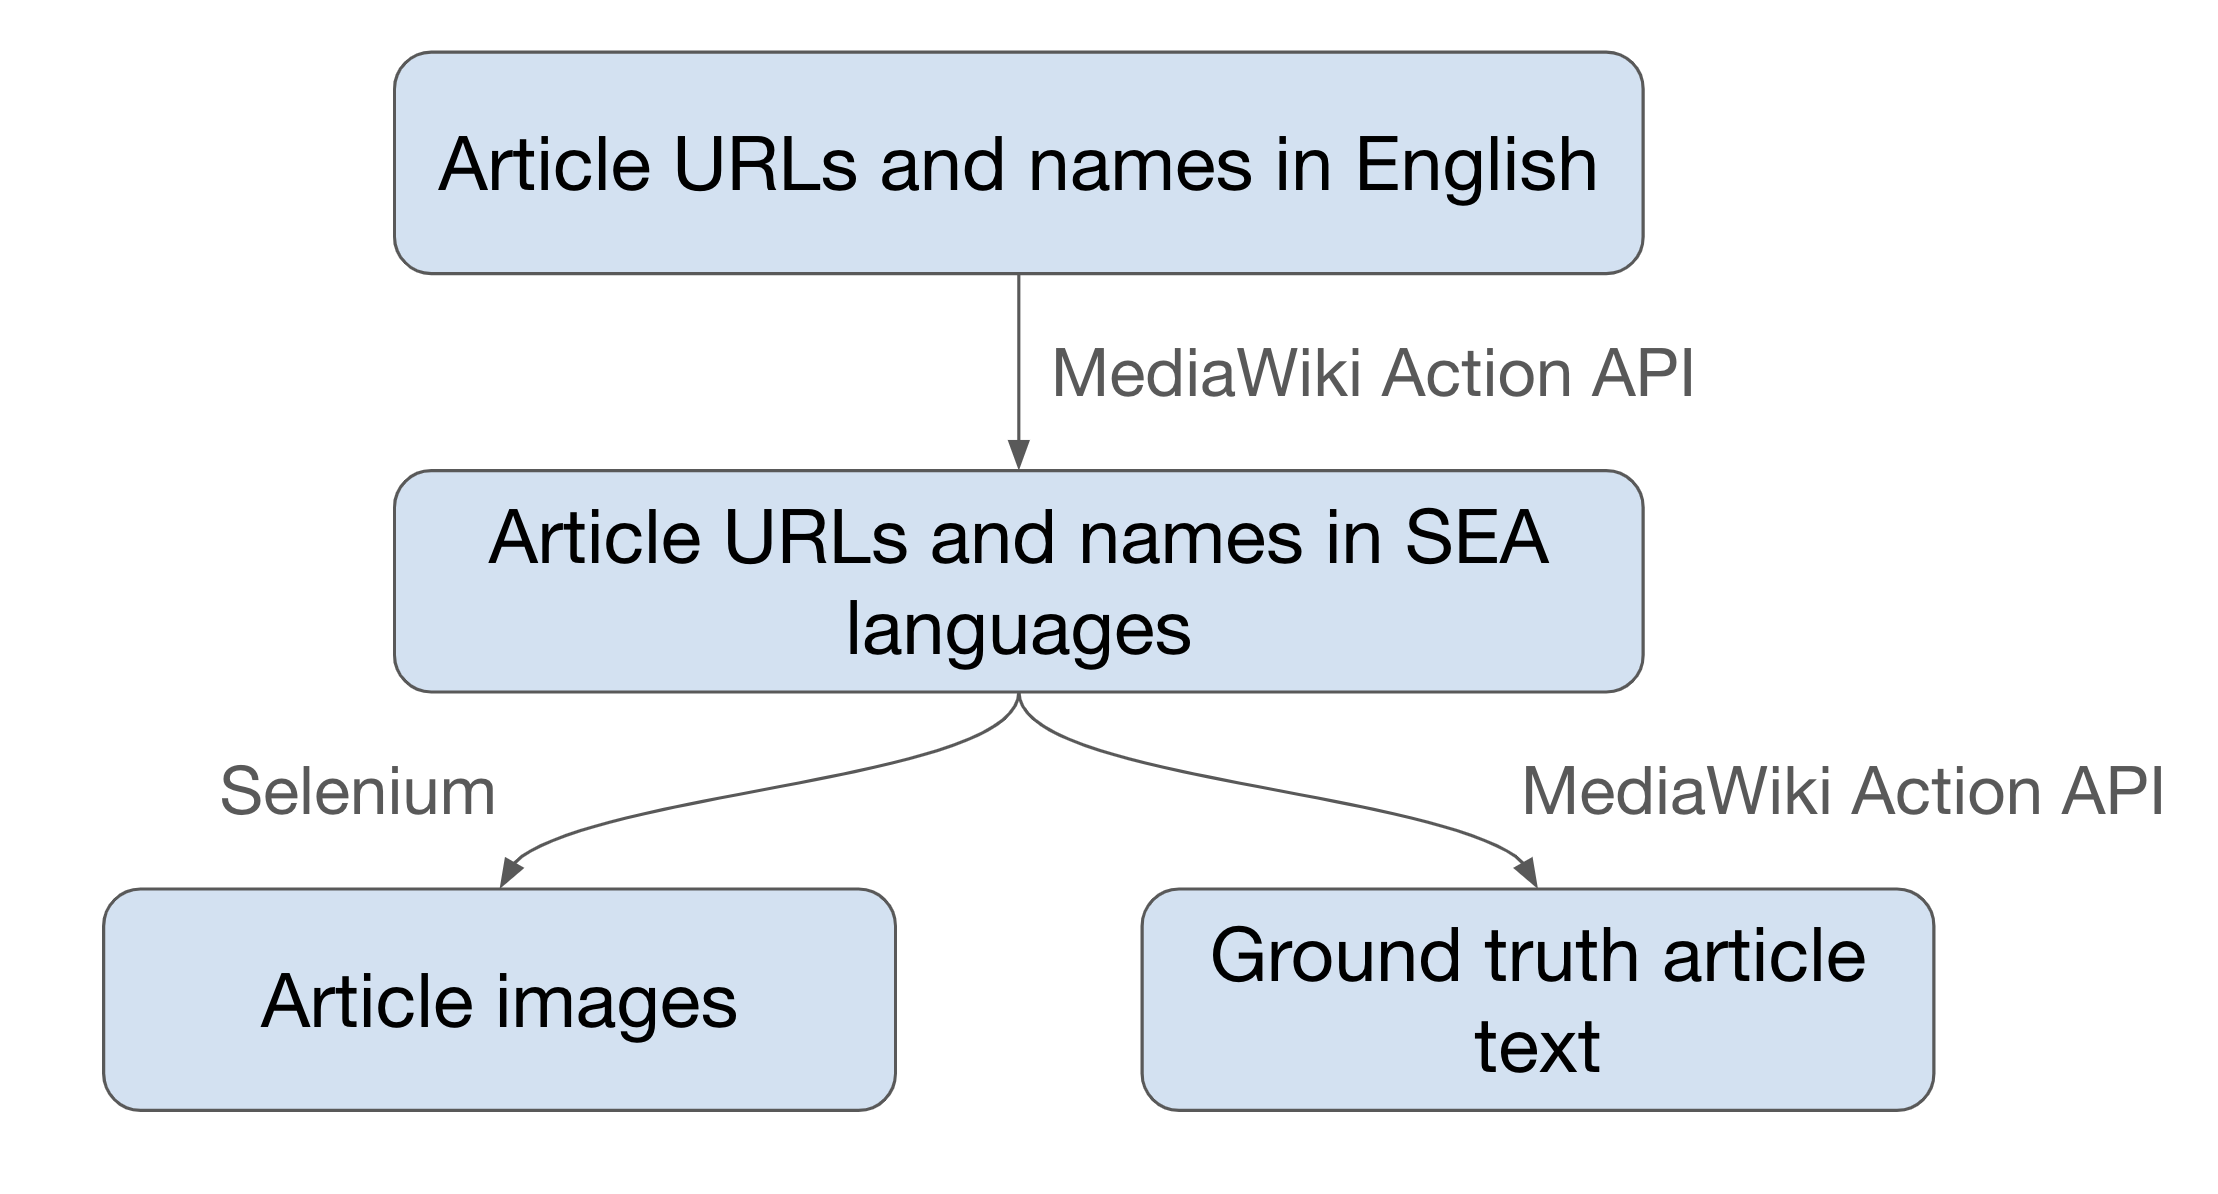
\includegraphics[width=0.6\textwidth]{images/data-collection.png}
    \caption{Pipeline for data collection from Wikipedia}
    \label{figure:data-collection}
\end{figure}

From the dataset of 100 Wikipedia articles, we collected article images and ground 
truth article text in our selected languages using Python, 
Selenium\footnote{\href{https://selenium-python.readthedocs.io}{Selenium} is a 
framework for automating web browsers, commonly used for web scraping by programmatically 
interacting with websites.}, and the MediaWiki Action API\footnote{The \href{https://www.mediawiki.org/wiki/API:Main_page}{MediaWiki Action API} allows 
access to wiki page operation features such as search and retrieval.}. Figure \ref{figure:data-collection} illustrates the overall pipeline 
for data collection. The detailed steps are as follows:

\begin{enumerate}
    \item Manually compile the dataset’s article names and URLs in English.
    \item Fetch the article names and URLs in Thai, Vietnamese, and Indonesian from the MediaWiki Action API.
    \item Download the article PDFs in all languages using Selenium.
    \item Convert the article PDFs into PNG images, with each image representing one page of the PDF.
    \item Download the article text into TXT files from the MediaWiki Action API.
\end{enumerate}

The end result is a real-world Wikipedia dataset with 3,590 English images, 1,450 Indonesian images, 1,925 Vietnamese images, and 1,011 Thai images.
Figure \ref{figure:real-world-data} presents sample collected images.

\begin{figure}[ht]
    \centering
    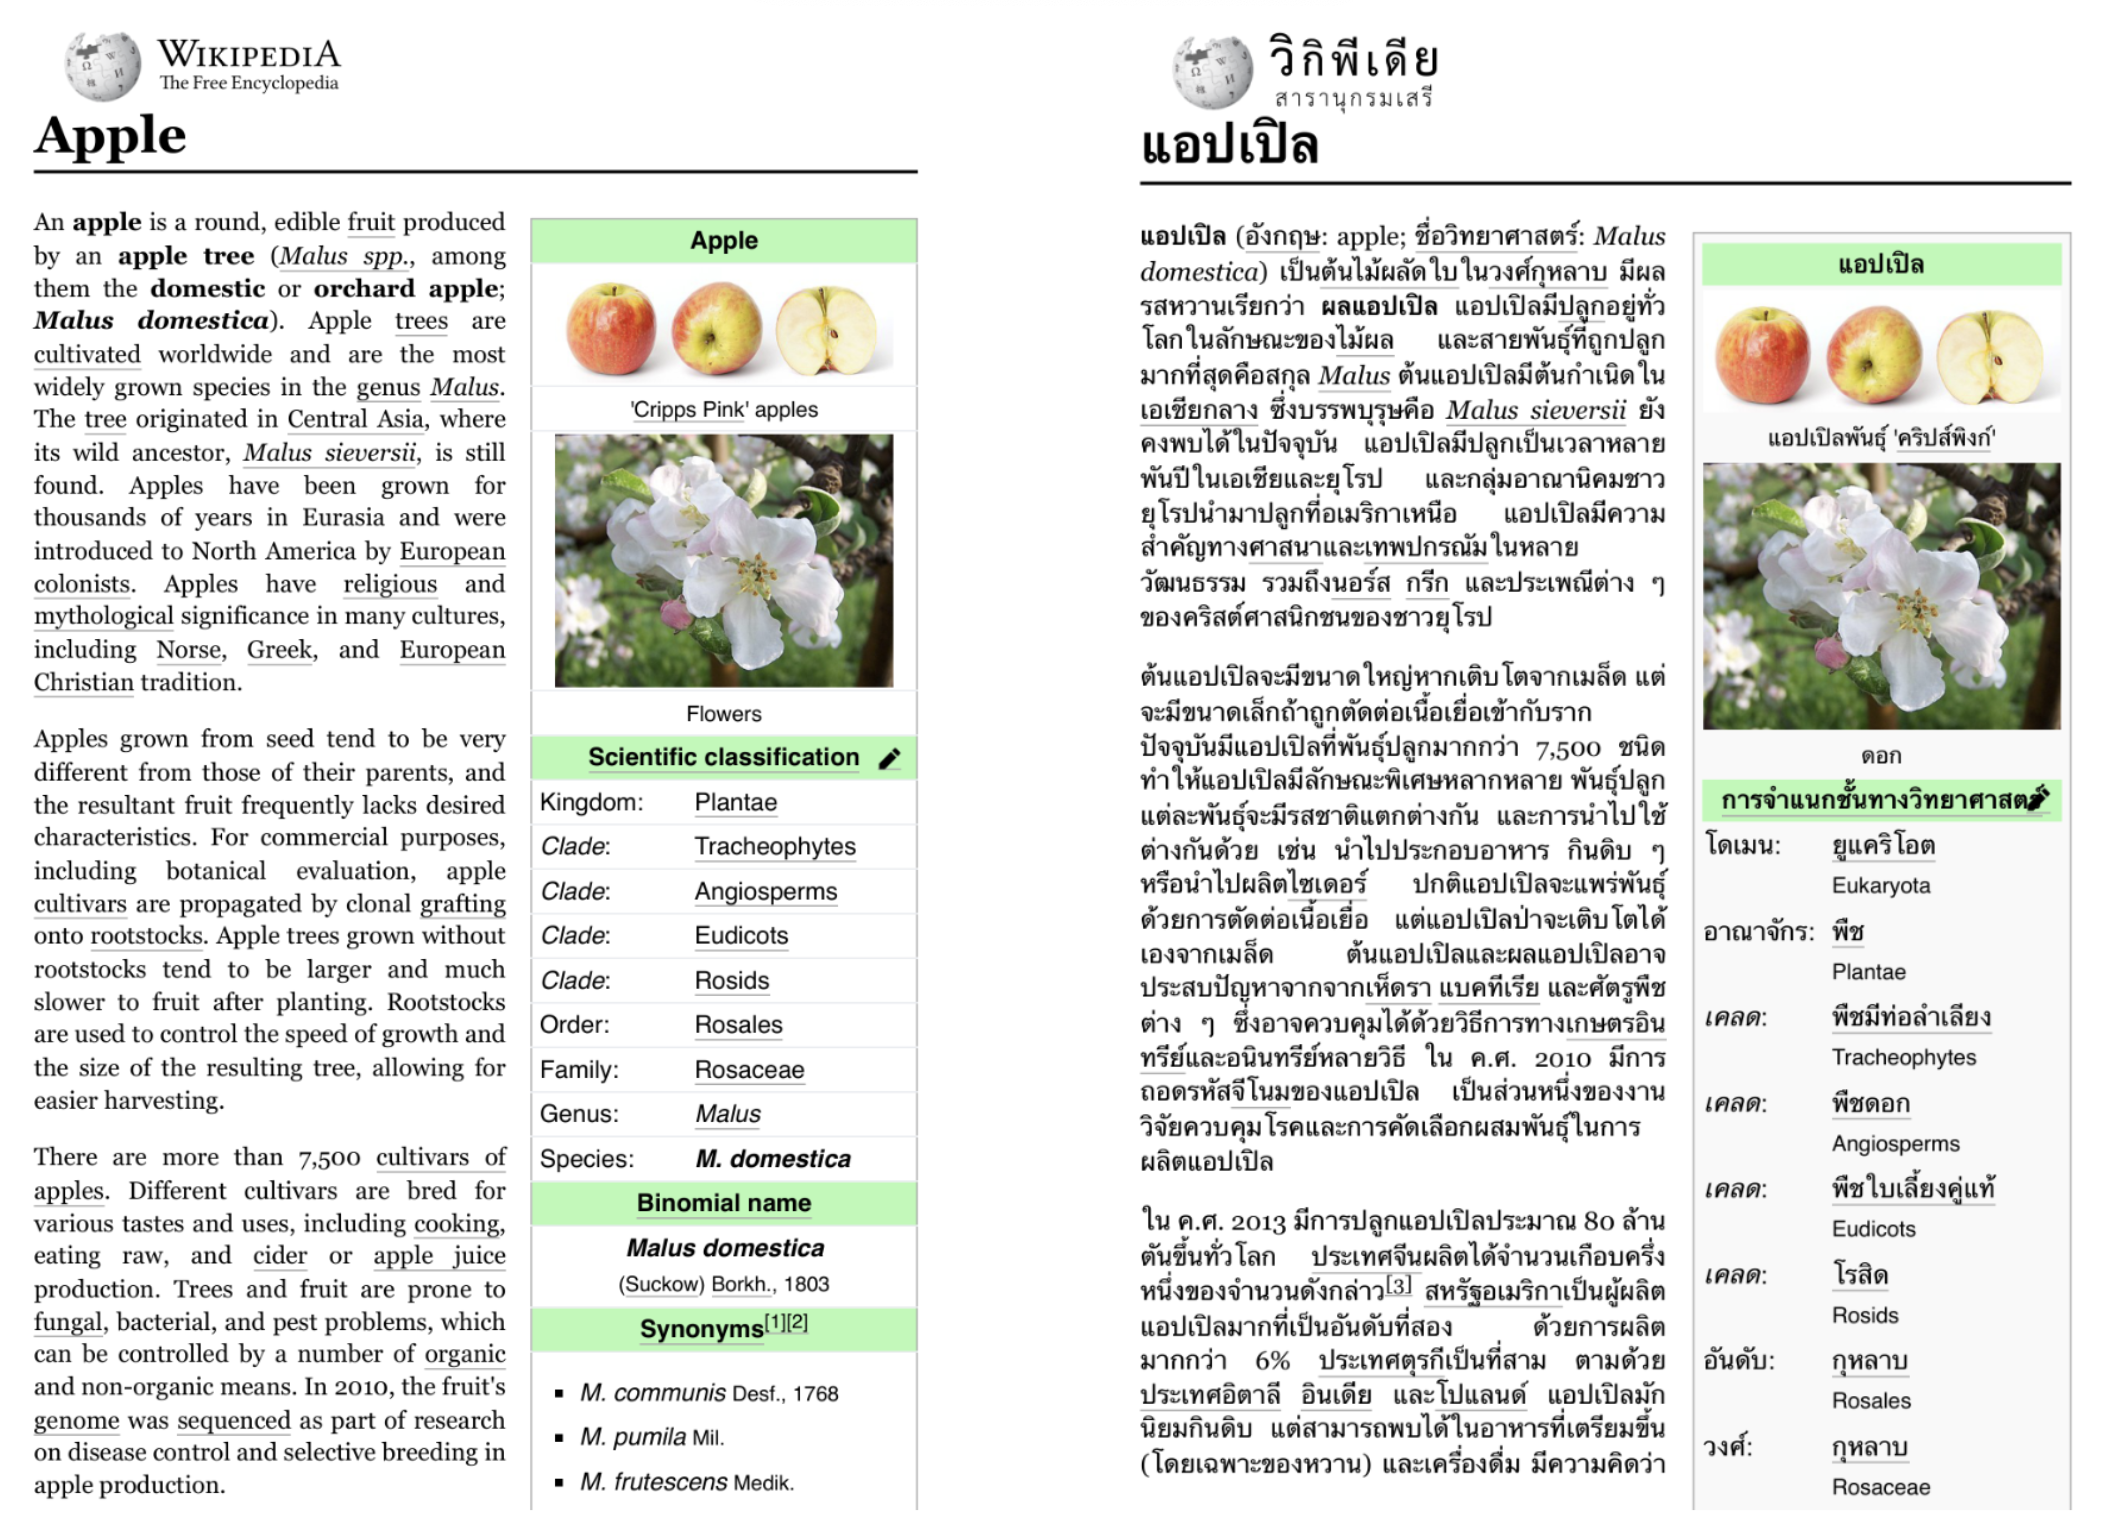
\includegraphics[width=0.65\textwidth]{images/real-world-data.png}
    \caption{Sample English and Thai images collected from Wikipedia}
    \label{figure:real-world-data}
\end{figure}

\subsection{OCR Evaluation} \label{section:ocr-evaluation}

\begin{figure}[ht]
    \centering
    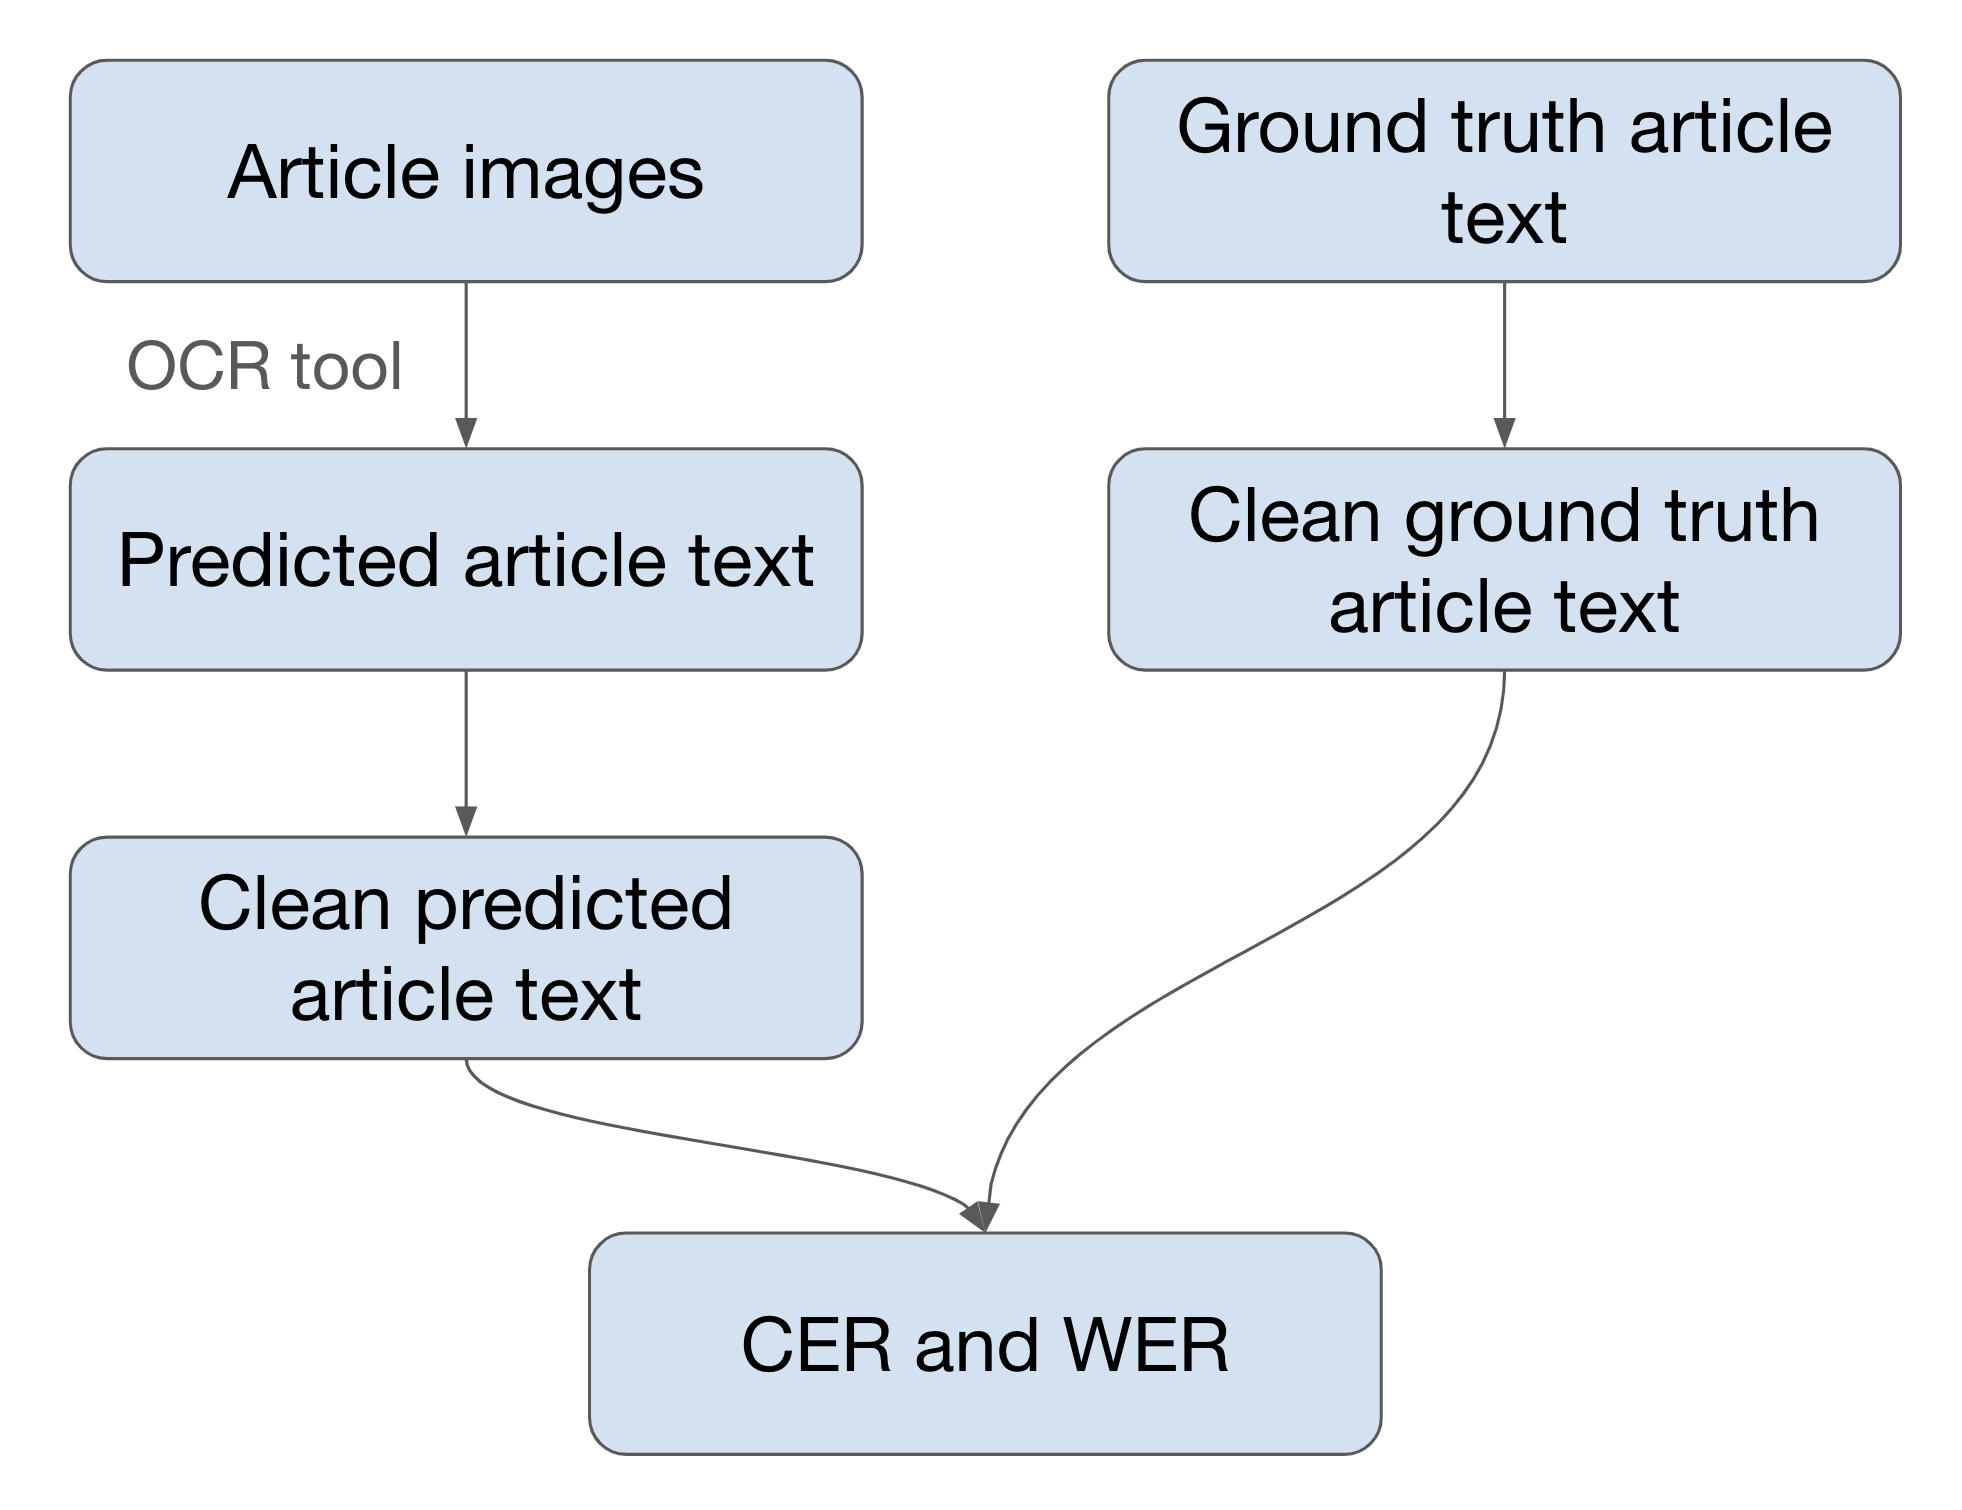
\includegraphics[width=0.6\textwidth]{images/ocr-evaluation.png}
    \caption{Pipeline for OCR evaluation}
    \label{figure:ocr-evaluation}
\end{figure}

After collecting the images and corresponding ground truth text, we ran the OCR tools and evaluated the CER and WER for each article.
Figure \ref{figure:ocr-evaluation} summarizes the overall pipeline for OCR evaluation. The detailed steps are as follows:

\begin{enumerate}
    \item \textbf{Apply OCR:} Apply the OCR tools on the article images.
\end{enumerate}

To run EasyOCR, Tesseract, and GOT on all 7,976 images, we used Slurm for job scheduling and execution on the SoC Compute Cluster at the School of Computing, National University of Singapore. Python and shell scripts were utilized to automate OCR execution.

\begin{enumerate}
    \setcounter{enumi}{1}
    \item \textbf{Data Cleaning:} Perform data cleaning on the predicted article text and ground truth article text.
\end{enumerate}

The raw predicted text generated by the OCR tools exhibited some consistent formatting issues.
For instance, Tesseract adds an additional space character after every predicted character.
The article images also included references and in-text citations, which are not present in the ground truth.
To address these issues, we performed data cleaning to align the output text more closely with the ground truth.

\begin{enumerate}
    \setcounter{enumi}{2}
    \item \textbf{Evaluation:} Compute the CER and WER between the predicted text and the ground truth text using JiWER\footnote{\href{https://pypi.org/project/jiwer/}{JiWER} is a Python package designed for fast calculation of CER and WER.}.
    \item \textbf{Data Validation:} Manually review articles with outlier CER values for incorrect ground truth text.
\end{enumerate}

To prevent erroneous results, we implemented a data validation step that automatically checked the CERs for each article.
Articles were flagged as outliers if their CER exceeded two standard deviations from the mean \parencite{cousineau-and-chartier-2010}. 
We manually reviewed these outlier articles for anomalies, resulting in the removal of around five articles per language, where the images and ground truth texts contained different content.

\section{Experiment 2: Benchmarking on Synthetic Data}

Unlike Experiment 1, Experiment 2 generates images from plain text for benchmarking. 
This approach allows us to introduce controlled distortions to the dataset, enabling an analysis of OCR robustness against noise on SEA languages and offering a different perspective on RQ1.
Additionally, using synthetic data minimizes annotation errors, allowing us to better isolate script-related errors (RQ2).

\subsection{Synthetic Data Generation}

Using the article text collected from Experiment 1, we generated synthetic article images with Python and WeasyPrint\footnote{\url{https://pypi.org/project/weasyprint/}}, a Python package for converting HTML pages into PDF documents.
To introduce font noise into the dataset, we randomly applied HTML tags to a specified ratio of space-separated words.
For instance, a \texttt{<b>} tag could be added randomly to make words appear in bold.
The following steps summarizes the process of data generation:

\begin{enumerate}
    \item To add noise, randomly apply HTML tags to a specified ratio of space-separated words.
    \item Generate synthetic article PDFs using the ground truth text collected from Experiment 1 with WeasyPrint.
    \item Convert the article PDFs into PNG images, with each image representing one page of the PDF.
\end{enumerate}

\subsection{OCR Evaluation on Different Types of Noise}

\begin{table}[ht]
    \centering
    \caption{Types of noise applied}
    \label{table:noises}
    \begin{tabular}{lcc}
        \toprule
        & HTML Tag & Ratio\\
        \midrule
        Bold & \texttt{<b>} & 0.3\\
        Italic & \texttt{<i>} & 0.3\\
        Link & \texttt{<a>} & 0.3\\
        Heading & \texttt{<h1>} & 0.03\\
        \bottomrule
    \end{tabular}
\end{table}

To investigate how different types of noise impact OCR performance (RQ1), we generated separate datasets, each containing a specific type of noise: bold, italic, link, or heading. 
The noise was randomly applied to a specified percentage of words in each dataset. 
Additionally, a control dataset without noise was created for comparison.

Table \ref{table:noises} summarizes the noise types, their corresponding HTML tags, and the percentage of words affected.
A smaller ratio was applied for headings because headings typically appear less frequently in natural text compared to other formatting elements like bold or italics.
Limiting the number of headings also helped reduce the number of pages generated, ensuring a more manageable dataset size.
Figure \ref{figure:noises} presents a sample synthetic image with different types of noise.

\begin{figure}[ht]
    \centering
    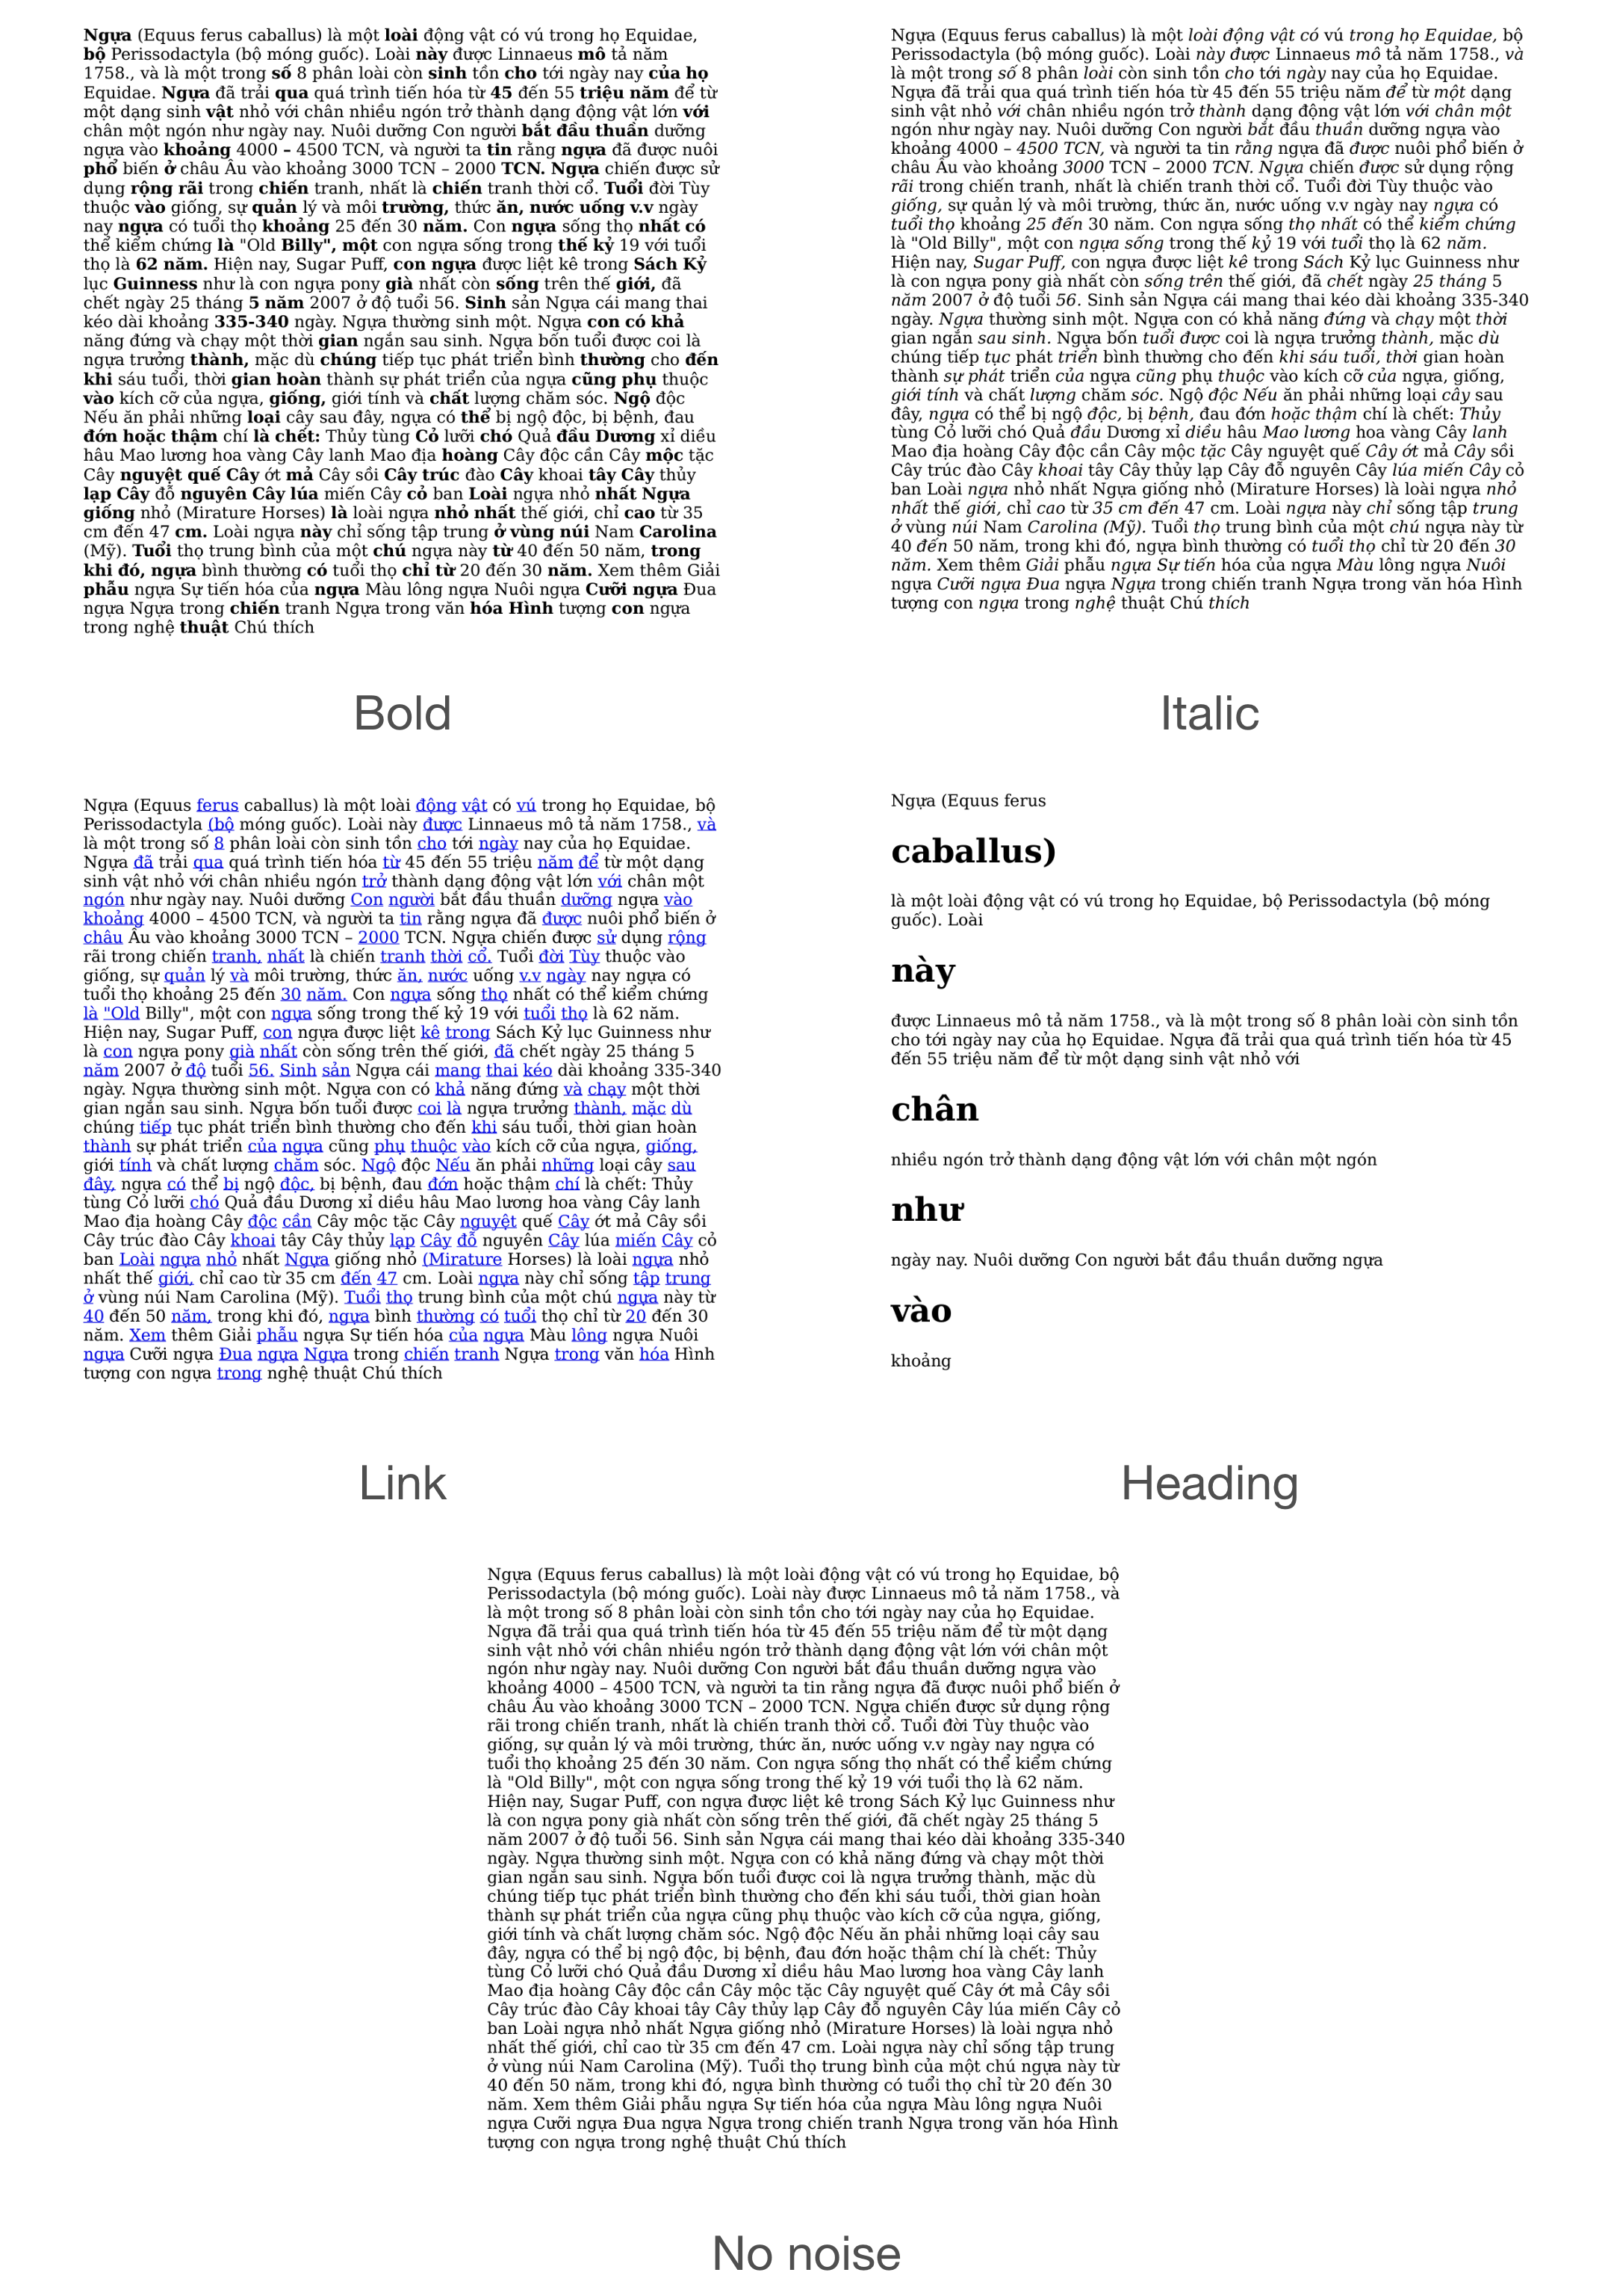
\includegraphics[width=0.8\textwidth]{images/noises.png}
    \caption{Sample synthetic image with different types of noise}
    \label{figure:noises}
\end{figure}

The selected noise types introduce formatting-based distortions commonly found in digital text and web-based content, posing unique challenges for OCR systems.
Bold and italic formatting, frequently used for emphasis in scanned documents and articles, may alter character shapes and affect recognition accuracy.
Links introduce underlining and color changes, which can interfere with OCR systems.
Headings, often bold and larger in size, may also impact recognition.
Evaluating these effects helps to assess OCR robustness in processing real-world digital text.

After generating the five separate datasets, we ran the OCR tools and evaluated their performance on each dataset, following the approach described in Section \ref{section:ocr-evaluation}.

\subsection{Error Classification by Character Type}

Another area of interest in Experiment 2 was the effect of unique script characteristics, such as diacritics and punctuation, on OCR accuracy (RQ2).
Using OCR results from the control dataset without noise, we categorized misclassifications by eight character types commonly found in English, Indonesian, Vietnamese, and Thai.

\begin{table}[ht]
    \centering
    \caption{Character types used for error classification}
    \label{table:character-types}
    \begin{tabular}{ll}
        \toprule
        & Included Characters\\
        \midrule
        Arabic digit & 0-9\\
        Latin letter & a-z, A-Z\\
        Latin letter with diacritic& à-ỹ, À-Ỹ\\
        Vietnamese special letter & đ, Đ\\
        Thai letter& {\fontspec{Tahoma} ก-ฮ}\\
        Special symbol& .,!?;:()-"–'—\$\%/\&+-=[]\\
        Whitespace& \textvisiblespace\\
        Other& \\
        \bottomrule
    \end{tabular}
\end{table}

We used the Levenshtein\footnote{\url{https://pypi.org/project/Levenshtein/}} Python package to identify edit operations (insertions, deletion, and substitutions) and classified misrecognized characters using RegEx\footnote{\url{https://docs.python.org/3/library/re.html}}. 
Table \ref{table:character-types} lists the character types we analyzed, with all uncategorized characters grouped under ``Other".

\section{Experiment 3: Fine-tuning for Vietnamese and Thai} \label{section:experiment-3}

To explore how fine-tuning can enhance OCR accuracy on SEA languages (RQ3), Experiment 3 fine-tunes GOT for Vietnamese and Thai and compares the fine-tuned model with EasyOCR and Tesseract. 
We chose to fine-tune for Vietnamese and Thai because GOT does not natively support these languages. 
Although GOT does not support Indonesian, we did not fine-tune for it, since the model already achieves state-of-the-art results for Indonesian, as demonstrated in the results from Experiment 1 (See Section \ref{section:ocr-accuracy-on-synthetic-data}). 

\subsection{Fine-tuning GOT}

\begin{figure}[ht]
    \centering
    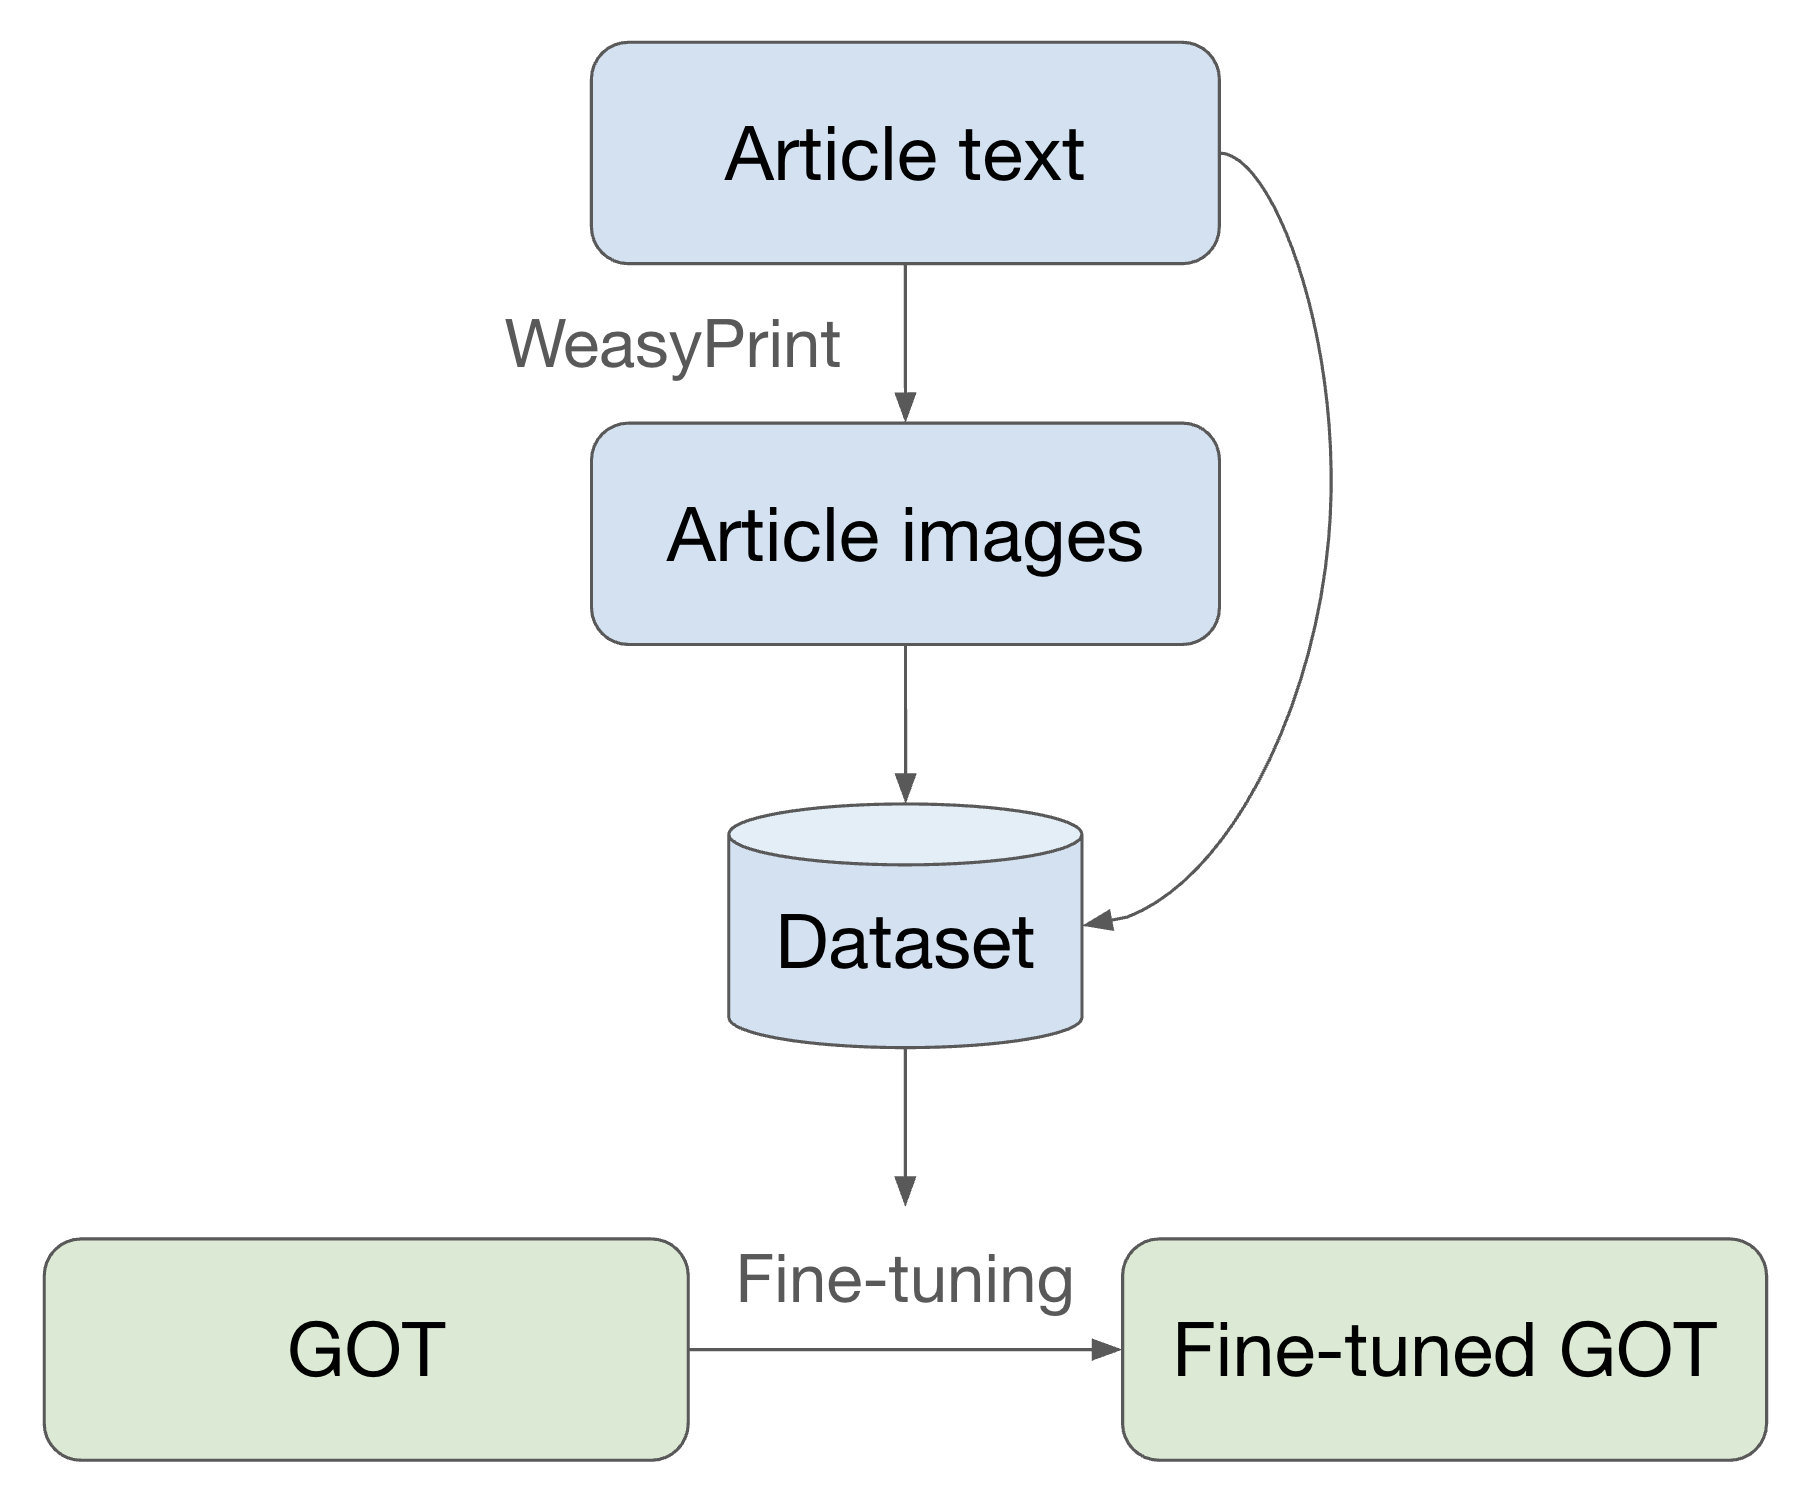
\includegraphics[width=0.6\textwidth]{images/fine-tuning.png}
    \caption{Pipeline for fine-tuning GOT}
    \label{figure:fine-tuning}
\end{figure}

Fine-tuning our model effectively required a large volume of high-quality data. 
To ensure the reliability of our training data, we generated additional synthetic data without noise. 
After collecting more plain text from Wikipedia, we created 960 images for training and 50 images for testing, for both Vietnamese and Thai.
To investigate how much training data is needed for effective fine-tuning, we randomly selected samples from the training dataset to create datasets with 50, 100, 200, 400, and 960 images. 
These sample sizes were chosen to follow an increasing scale, approximating diminishing returns as data size increases.
For each dataset, the same base model (GOT) was fine-tuned for three epochs, resulting in different fine-tuned models based on the varying dataset sizes.

For fine-tuning, we used SWIFT\footnote{\url{https://github.com/modelscope/ms-swift}}, a user-friendly framework that supports fine-tuning GOT\footnote{\url{https://github.com/modelscope/ms-swift/issues/2122}}. 
Using a single NVIDIA Titan V GPU on the SoC Compute Cluster, we fine-tuned our model using Low-Rank Adaptation (LoRA), which optimizes only small adapter layers while keeping the pre-trained model weights frozen \parencite{hu-etal-2021}.
This approach allows for efficient fine-tuning with reduced memory and computational costs.

\subsection{OCR Evaluation on Fine-tuned GOT}

We ran each fine-tuned GOT model on the test dataset and evaluated their performance, following the approach described in Section \ref{section:ocr-evaluation}.
We also ran EasyOCR and Tesseract on the test dataset for comparison.

\chapter{Results and Discussion}

In this chapter, we present and analyze the results of the experiments, evaluating their significance and discussing the insights gained in relation to the research questions.

\section{RQ1: How do popular OCR tools perform on SEA scripts?}

\subsection{OCR Accuracy on Wikipedia Screenshots} \label{section:ocr-accuracy-on-wikipedia-screenshots}

\begin{table}[ht]
    \centering
    \caption{Average Character and Word Error Rate on Wikipedia screenshots}
    \label{table:ocr-accuracy-on-real-world-data}
    \begin{tabular}{lcccccc}
        \toprule
        & \multicolumn{3}{c}{Character Error Rate} & \multicolumn{3}{c}{Word Error Rate}\\
        \cmidrule(lr){2-4}\cmidrule(lr){5-7}
        & EasyOCR & Tesseract & GOT & EasyOCR & Tesseract & GOT\\
        \midrule
        English & \textbf{0.21} & \textbf{0.21} & 0.67 & \textbf{0.27} & 0.29 & 0.67\\
        Indonesian & \textbf{0.28} & \textbf{0.28} & 0.61 & \textbf{0.36} & 0.42 & 0.71\\
        Vietnamese & 0.47 & \textbf{0.38} & - & 0.45 & \textbf{0.39} & -\\
        Thai & \textbf{0.35} & 0.55 & - & \textbf{1.45} & \textbf{1.45} & -\\
        \bottomrule
    \end{tabular}
\end{table}

Table \ref{table:ocr-accuracy-on-real-world-data} lists the results from benchmarking the OCR tools on real-world Wikipedia screenshots (Experiment 1).
A lower Character Error Rate (CER) and Word Error Rate (WER) implies better OCR accuracy.
Bolded numbers highlight the best-performing tool for each metric and language. Our observations are as follows:

\begin{itemize}
    \item \textbf{Latin scripts achieved the best performance.} When comparing performance across script types, Latin scripts (English and Indonesian) had the lowest average CER of 0.38, followed by Latin scripts with diacritics (Vietnamese) with an average CER of 0.42 and Brahmic scripts (Thai) with 0.45. These results align with findings from previous studies, which have shown that OCR tools tend to perform best on Latin-based scripts \parencite{hegghammer-2022,ignat-etal-2022}.
    \item \textbf{EasyOCR achieved the best overall performance on the Wikipedia screenshots among the OCR tools,} with an average CER of 0.33 across all languages. This was followed by Tesseract with an average CER of 0.35, and GOT with 0.64. 
    \item \textbf{WER may not be a reliable metric for non-segmented scripts.} Thai had a particularly high average WER of 1.45, as Thai is a non-segmented script that lacks explicit word boundaries. This characteristic makes word-level evaluation more challenging for OCR systems.
\end{itemize}

\subsubsection{Limitations of Wikipedia Screenshots}

\begin{figure}[ht]
    \centering
    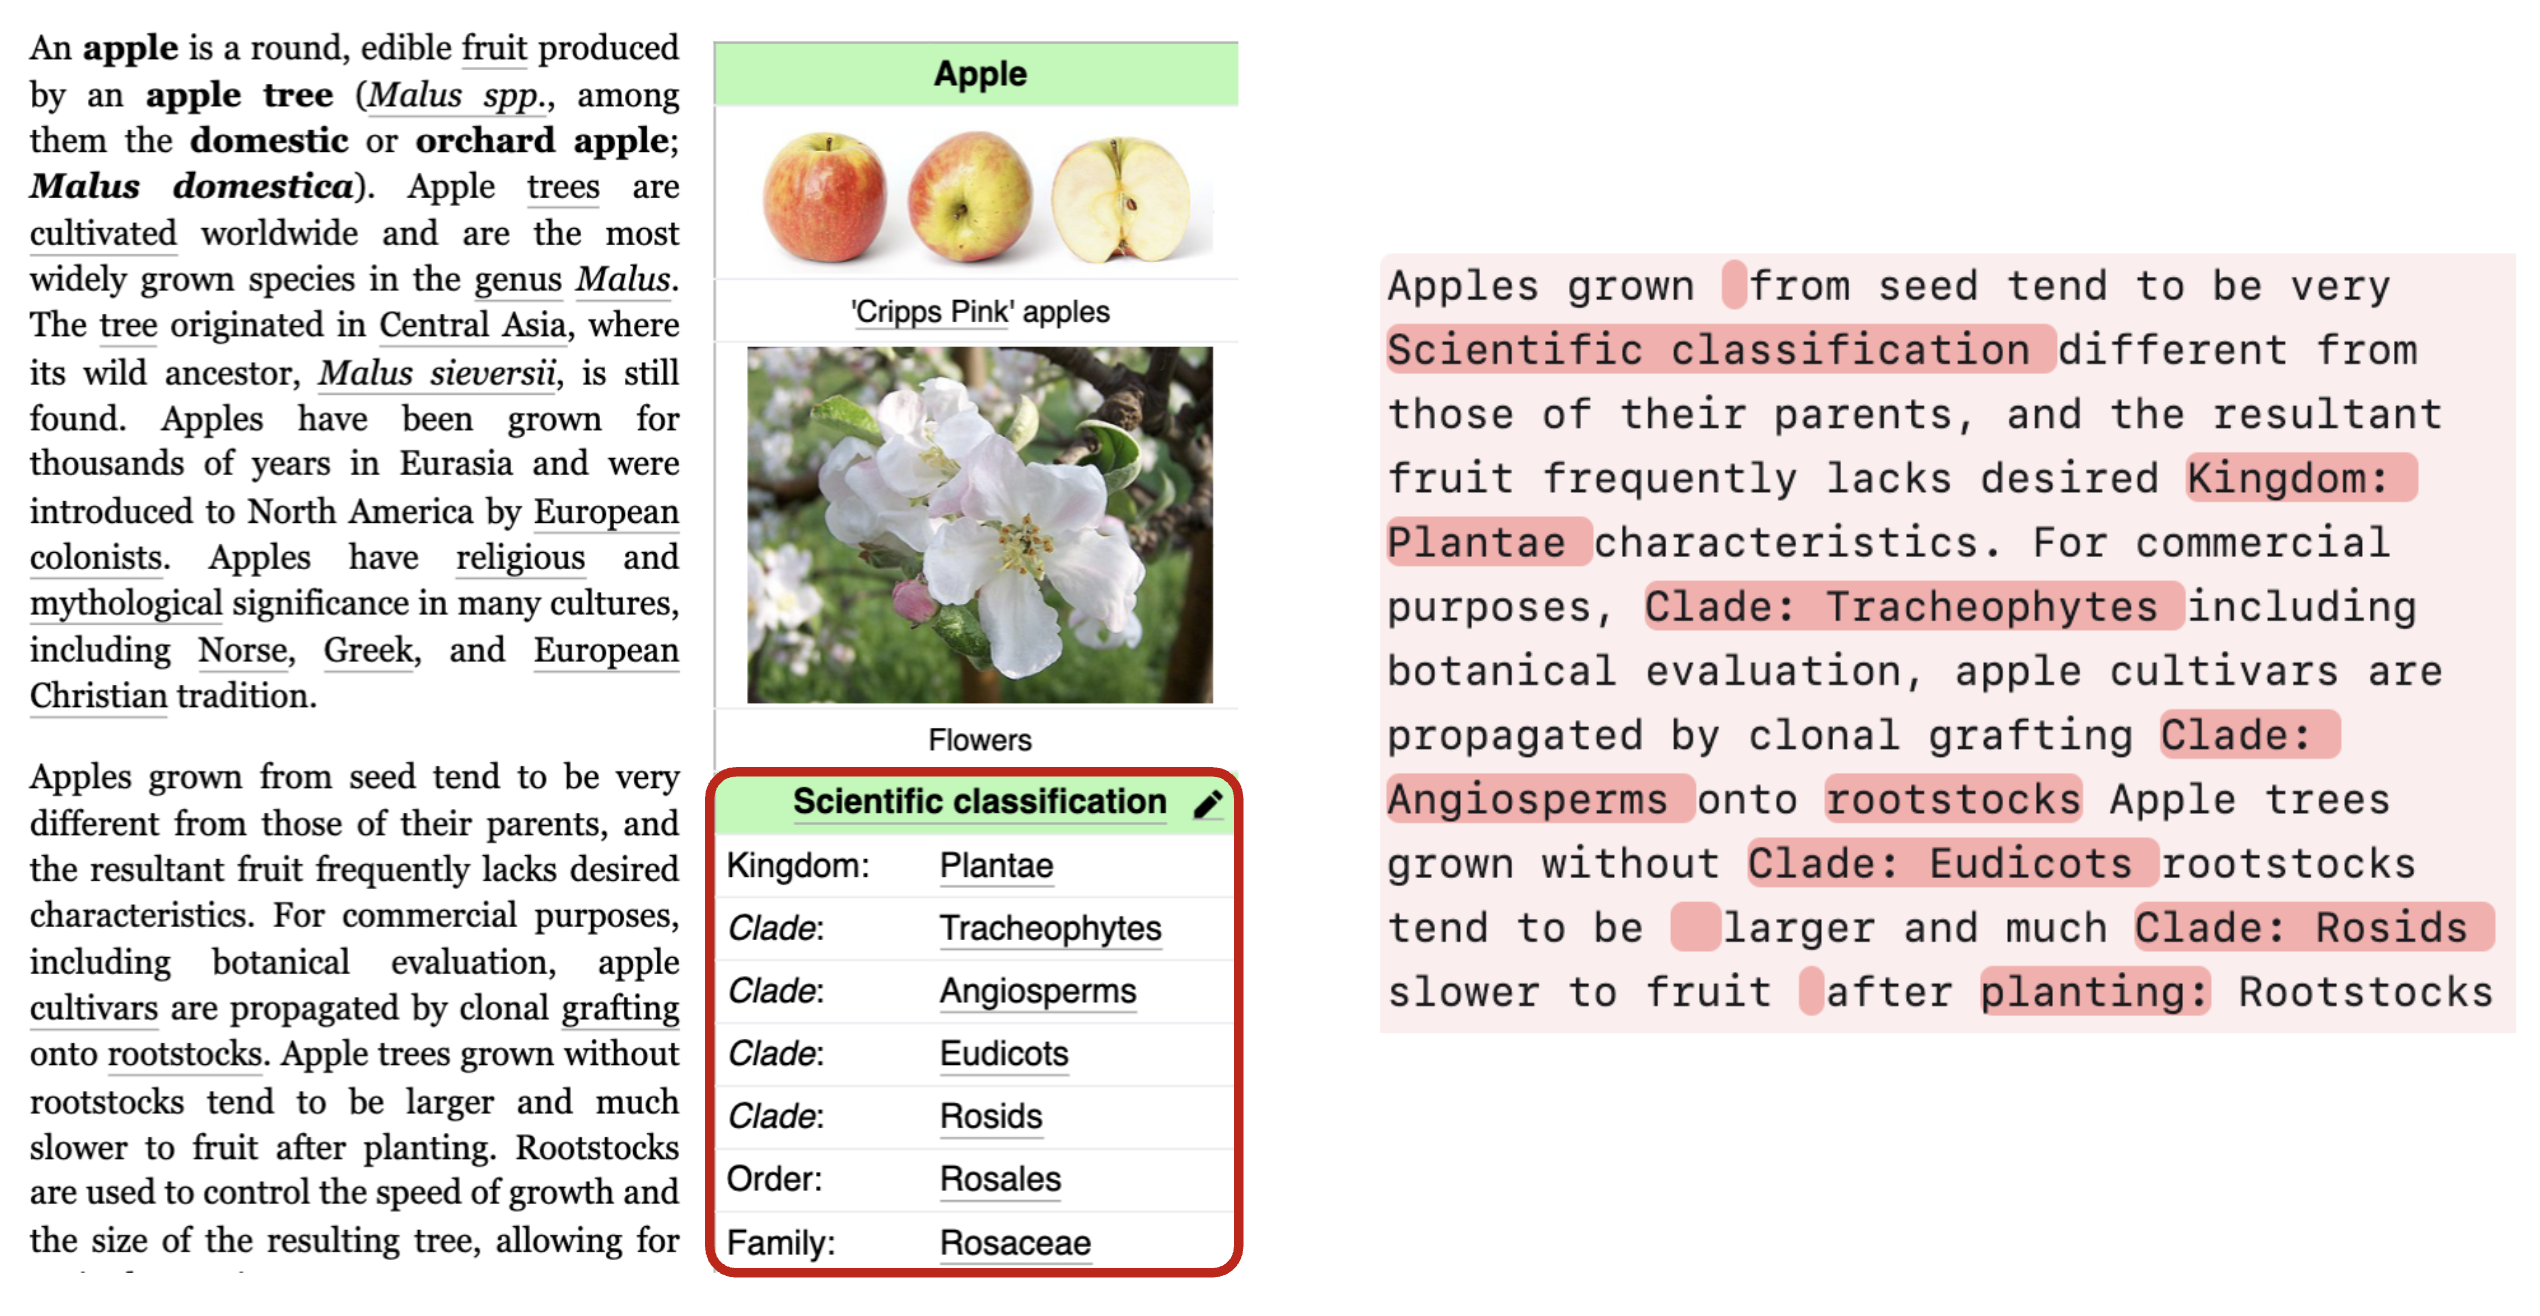
\includegraphics[width=0.8\textwidth]{images/wikipedia-limitations.png}
    \caption{Table in Wikipedia articles that interferes with OCR results}
    \label{figure:wikipedia-limitations}
\end{figure}

Wikipedia articles often have complex layouts and multi-modal elements, such as tables and embedded text in images, that interfere with OCR results.
For example, in Figure \ref{figure:wikipedia-limitations}, the OCR tool mistakenly recognized the text inside a table as part of the main article text, interweaving it with the surrounding content.
Since the ground truth article text collected from the MediaWiki Action API does not include table content, this discrepancy contributed to higher CERs and WERs in the Wikipedia screenshot results.

Accurately recognizing such complex layouts in practical settings requires document layout analysis.
Although layout analysis is beyond the scope of this study, this limitation highlights its importance in processing modern digital documents.
Future work on document recognition can explore layout-aware approaches.

One possible workaround is to use Selenium to generate bounding boxes around the main article text, restricting OCR to only those regions.
However, we felt this would not accurately reflect the challenges in recognizing real-world digital documents, which often contain complex layouts and multi-modal elements.
To preserve the realism of the task, we chose to retain the raw OCR results from Wikipedia screenshots. 
A separate Experiment 2 using noise-free synthetic data was also conducted to better isolate errors specifically related to character recognition.

\subsection{OCR Accuracy on Synthetic Data} \label{section:ocr-accuracy-on-synthetic-data}

\begin{table}[ht]
    \centering
    \caption{Average Character and Word Error Rate on synthetic data}
    \label{table:ocr-accuracy-on-synthetic-data}
    \begin{tabular}{lcccccc}
        \toprule
        & \multicolumn{3}{c}{Character Error Rate} & \multicolumn{3}{c}{Word Error Rate}\\
        \cmidrule(lr){2-4}\cmidrule(lr){5-7}
        & EasyOCR & Tesseract & GOT & EasyOCR & Tesseract & GOT\\
        \midrule
        English & 0.03 & 0.02 & \textbf{0.01} & 0.09 & \textbf{0.04} & \textbf{0.04}\\
        Indonesian & 0.02 & 0.02 & \textbf{0.01} & 0.09 & 0.06 & \textbf{0.05}\\
        Vietnamese & 0.10 & \textbf{0.03} & - & 0.17 & \textbf{0.04} & -\\
        Thai & \textbf{0.07} & 0.09 & - & 0.68 & \textbf{0.64} & -\\
        \bottomrule
    \end{tabular}
\end{table}

Table \ref{table:ocr-accuracy-on-synthetic-data} presents the results from benchmarking the OCR tools on synthetic documents without noise (Experiment 2). Our observations are as follows:

\begin{itemize}
    \item \textbf{Latin scripts achieved the best results on synthetic data,} followed by Latin scripts with diacritics and Brahmic scripts. This finding is consistent with the trend observed in the benchmarking of real-world Wikipedia data.
    \item \textbf{The OCR tools performed better on synthetic data than on Wikipedia screenshots.} All metrics showed an average decrease in error rate by 0.34. This observation aligns with the findings from \textcite{ignat-etal-2022} and \textcite{hegghammer-2022}.
    \item \textbf{GOT and Tesseract performed well on synthetic data.} 
    On synthetic data, GOT achieved the best results with an average CER of 0.01, followed by Tesseract with 0.04 and EasyOCR with 0.05.
    This contrasts with the results from the Wikipedia screenshots.
    This findings suggest that GOT and Tesseract may not be robust to noise, but can achieve high accuracy in noise-free environments, as further discussed in Section \ref{section:impact-of-noise}.
\end{itemize}

\subsection{Impact of Noise on OCR Accuracy} \label{section:impact-of-noise}

\begin{table}[ht]
    \centering
    \caption{Impact of noise on EasyOCR's accuracy}
    \label{table:noise-easy-ocr}
    \begin{tabular}{lrrrrr}
        \toprule
        & No Noise & Bold & Italic & Link & Heading\\
        & CER & \% Change & \% Change & \% Change & \% Change\\
        \midrule
        English & 0.03 & \greentc{-7.1\%} & 0.0\% & \redtc{3.6\%} & \greentc{-7.1\%}\\
        Indonesian & 0.02 & \greentc{-5.6\%} & 0.0\% & \redtc{22.2\%} & \greentc{-5.6\%}\\
        Vietnamese & 0.10 & \greentc{-1.0\%} & \greentc{-1.9\%} & \greentc{-6.7\%} & \greentc{-11.5\%}\\
        Thai & 0.07 & 0.0\% & 0.0\% & \redtc{7.2\%} & 0.0\%\\
        \bottomrule
    \end{tabular}
\end{table}

\begin{table}[ht]
    \centering
    \caption{Impact of noise on Tesseract's accuracy}
    \label{table:noise-tesseract}
    \begin{tabular}{lrrrrr}
        \toprule
        & No Noise & Bold & Italic & Link & Heading\\
        & CER & \% Change & \% Change & \% Change & \% Change\\
        \midrule
        English & 0.02 & \greentc{-4.2\%} & 0.0\% & 0.0\% & \redtc{8.3\%}\\
        Indonesian & 0.02 & 0.0\% & 0.0\% & 0.0\% & \redtc{21.7\%}\\
        Vietnamese & 0.03 & 0.0\% & \redtc{3.8\%} & \redtc{3.8\%} & \redtc{26.9\%}\\
        Thai & 0.09 & \redtc{3.2\%} & 0.0\% & \redtc{5.4\%} & \redtc{4.3\%}\\
        \bottomrule
    \end{tabular}
\end{table}

\begin{table}[ht]
    \centering
    \caption{Impact of noise on GOT's accuracy}
    \label{table:noise-got}
    \begin{tabular}{lrrrrr}
        \toprule
        & No Noise & Bold & Italic & Link & Heading\\
        & CER & \% Change & \% Change & \% Change & \% Change\\
        \midrule
        English & 0.01 & \redtc{27.3\%} & \redtc{36.4\%} & \greentc{-18.2\%} & \redtc{218.2\%}\\
        Indonesian & 0.01 & \redtc{9.1\%} & \redtc{18.2\%} & \redtc{36.4\%} & \redtc{63.6\%}\\
        \bottomrule
    \end{tabular}
\end{table}

Table \ref{table:noise-easy-ocr} presents the results from benchmarking EasyOCR on synthetic documents with noise (Experiment 2).
Using the noise-free dataset as the baseline, we calculated the percent change for each noise type and language. 
A negative percent change indicates that the error rate decreased with the added noise, while a positive percent change indicates that the error rate increased. To visually distinguish these changes, positive values are highlighted in red and negative values in green. 
Similar results for Tesseract and GOT are shown in Table \ref{table:noise-tesseract} and Table \ref{table:noise-got} respectively. 
Our observations from these results are as follows:

\begin{itemize}
    \item \textbf{EasyOCR was the most robust to noise among the OCR tools.}
    EasyOCR had the lowest average percent change of -0.8\%, followed by Tesseract with an average percent change of 4.6\% and GOT with 48.9\%. Notably, adding noise improved the performance of EasyOCR, suggesting that it may be particularly well-suited to handle noisy data.
    \item \textbf{Tesseract and GOT were sensitive to noise.} This finding aligns with the results from Section \ref{section:ocr-accuracy-on-synthetic-data}, where Tesseract and GOT performed well on synthetic data but struggled with real-world Wikipedia screenshots, which contain noise and complex layouts.
    \item \textbf{Heading noise impacted the OCR tools the most,} with an average percent change of 31.9\%, followed by italic noise (5.6\%), link noise (5.4\%), and bold noise (2.2\%). This result indicates that larger font sizes with bold formatting, as seen in the heading noise, pose the greatest challenge to OCR systems.
\end{itemize}

\subsubsection{Limitations of Noise Types}

The selected noise types in our experiment are commonly found in digital text and web-based content but may not fully represent the range of noise found in other document types.
For instance, scanned physical documents can contain noise from poor lighting, rotations, and blurry scans \parencite{hegghammer-2022}. 
Additional artificial noise types could be incorporated in future studies, depending on the specific goals of the research.

\subsection{Runtime}

\begin{table}[ht]
    \caption{Average OCR runtime per page (seconds)}
    \label{table:runtime}
    \centering
    \begin{tabular}{lccc}
        \toprule
        & EasyOCR & Tesseract & GOT\\ 
        \midrule
        English & \textbf{3.2} & 11.7 & 24.3\\
        Indonesian & \textbf{2.9} & 13.2 & 31.4\\
        Vietnamese & \textbf{3.9} & 11.8 & -\\
        Thai & \textbf{2.3} & 16.8 & -\\
        \bottomrule
    \end{tabular}
\end{table}

Table \ref{table:runtime} presents the average OCR runtime per page, with the bolded numbers highlighting the fastest tool for each language. 
The runtimes were recorded when running the OCR tools on noise-free synthetic data (Experiment 2) on the SoC Compute Cluster. 
We observed that \textbf{EasyOCR is the fastest OCR tool,} with an average runtime of 3.1 seconds, followed by Tesseract at 13.4 seconds and GOT at 27.9 seconds.

\section{RQ2: What script-related challenges affect OCR accuracy on SEA languages?}

\subsection{Latin Scripts}

\begin{table}[ht]
    \caption{Error classification by character type in English articles}
    \label{table:error-classification-english}
    \centering
    \begin{tabular}{lrrrr}
        \toprule
        & \multirow{2}{*}{Count} & EasyOCR & Tesseract & GOT\\
        & & \% Missed & \% Missed & \% Missed\\
        \midrule
        Arabic digit & 38,324 & \cellcolor{LightRed!1}0.7\% & \cellcolor{LightRed!2}1.9\% & 0.3\%\\
        Latin letter & 1,546,964 & \cellcolor{LightRed!1}1.3\% & \cellcolor{LightRed!2}1.8\% & 0.4\%\\
        Latin letter with diacritic & 452 & \cellcolor{LightRed!100}100.0\% & \cellcolor{LightRed!56}56.0\% & \cellcolor{LightRed!16}15.9\%\\
        Special symbol & 55,110 & \cellcolor{LightRed!30}29.5\% & \cellcolor{LightRed!4}3.7\% & \cellcolor{LightRed!4}4.3\%\\
        Whitespace & 317,587 & \cellcolor{LightRed!5}4.9\% & \cellcolor{LightRed!4}4.3\% & \cellcolor{LightRed!4}3.6\%\\
        Other & 1,562 & \cellcolor{LightRed!104}103.6\% & \cellcolor{LightRed!93}92.6\% & \cellcolor{LightRed!128}127.9\%\\
        \bottomrule
    \end{tabular}
\end{table}

\begin{table}[ht]
    \caption{Error classification by character type in Indonesian articles}
    \label{table:error-classification-indonesian}
    \centering
    \begin{tabular}{lrrrr}
        \toprule
        & \multirow{2}{*}{Count} & EasyOCR & Tesseract & GOT\\
        & & \% Missed & \% Missed & \% Missed\\
        \midrule
        Arabic digit & 24,947 & 0.4\% & \cellcolor{LightRed!2}1.8\% & 0.2\%\\
        Latin letter & 1,208,707 & \cellcolor{LightRed!1}0.5\% & \cellcolor{LightRed!2}1.8\% & 0.4\%\\
        Latin letter with diacritic & 276 & \cellcolor{LightRed!7}7.2\% & \cellcolor{LightRed!100}100.0\% & \cellcolor{LightRed!17}16.7\%\\
        Special symbol & 38,980 & \cellcolor{LightRed!23}22.9\% & \cellcolor{LightRed!5}4.9\% & \cellcolor{LightRed!1}1.4\%\\
        Whitespace & 207,556 & \cellcolor{LightRed!5}4.8\% & \cellcolor{LightRed!5}5.1\% & \cellcolor{LightRed!4}4.1\%\\
        Other & 1,262 & \cellcolor{LightRed!94}94.4\% & \cellcolor{LightRed!100}99.6\% & \cellcolor{LightRed!65}64.8\%\\
        \bottomrule
    \end{tabular}
\end{table}

Table \ref{table:error-classification-english} presents the results of classifying errors by character type in the benchmark on English synthetic data without noise (Experiment 2). 
Results on Indonesian articles are shown in Table \ref{table:error-classification-indonesian}.
The ``Count" column lists the number of characters belonging to each character type in the ground truth text.
The remaining columns show the percentage of characters misclassified by each OCR tool.

Notably, these percentages can exceed 100\%, as demonstrated in Table \ref{table:error-classification-english} under the ``Other" character type.
This is similar to how CERs can exceed 1.
The reason for this is that the misclassifications are identified using edit operations, which include substitutions, deletions, and insertions. 
If the OCR tool incorrectly inserts additional characters, the number of misclassified characters can surpass the ground truth.

Our observations from the results on benchmarked Latin scripts are as follows:

\begin{itemize}
    \item \textbf{Latin letters, Arabic digits, and whitespaces achieved high accuracies.} These three character types accounted for 97\% of all characters in both English and Indonesian texts.
    \item \textbf{OCR tools for English and Indonesian struggled more with Latin letters containing diacritics than those without diacritics,} as evidenced by the higher error rates for diacritical characters.
    One possible explanation is that the OCR models were not trained on enough diacritical marks, which is reflected in their low frequency in the English and Indonesian datasets.

    In particular, EasyOCR and Tesseract misclassified all Latin characters with diacritics for English and Indonesian respectively, suggesting that their language-specific models were not trained to recognize diacritics.
\end{itemize}

\subsection{Latin Scripts with Diacritics}

\begin{table}[ht]
    \caption{Error classification by character type in Vietnamese articles}
    \label{table:error-classification-vietnamese}
    \centering
    \begin{tabular}{lrrr}
        \toprule
        & \multirow{2}{*}{Count} & EasyOCR & Tesseract\\
        & & \% Missed & \% Missed\\
        \midrule
        Arabic digit & 31,473 & \cellcolor{LightRed!1}1.1\% & \cellcolor{LightRed!2}2.2\% \\
        Latin letter & 916,667 & \cellcolor{LightRed!8}8.5\% & \cellcolor{LightRed!2}1.8\% \\
        Latin letter with diacritic & 294,406 & \cellcolor{LightRed!15}14.9\% & \cellcolor{LightRed!2}1.9\% \\
        Vietnamese special letter & 30,903 & \cellcolor{LightRed!4}4.2\% & \cellcolor{LightRed!2}1.8\% \\
        Special symbol & 41,655 & \cellcolor{LightRed!25}25.4\% & \cellcolor{LightRed!3}3.1\% \\
        Whitespace & 367,936 & \cellcolor{LightRed!11}10.9\% & \cellcolor{LightRed!5}5.3\% \\
        Other & 1,909 & \cellcolor{LightRed!105}105.4\% & \cellcolor{LightRed!89}88.6\% \\
        \bottomrule
    \end{tabular}
\end{table}

Table \ref{table:error-classification-vietnamese} presents the results of classifying errors in the benchmark on Vietnamese data without noise (Experiment 2). 
We observed that \textbf{Tesseract achieved high accuracies in recognizing Vietnamese characters.} 
Vietnamese characters, which make up 74\% of the dataset, consist of Latin letters with and without diacritics, as well as a special character (đ, Đ) categorized under ``Vietnamese special letter".
Only 2\% of these Vietnamese characters were misclassified by Tesseract, which is similar to the performance of English models in recognizing Latin letters.
In contrast, EasyOCR struggled more with diacritical characters.

\subsection{Brahmic Scripts}

\begin{table}[ht]
    \caption{Error classification by character type in Thai articles}
    \label{table:error-classification-thai}
    \centering
    \begin{tabular}{lrrr}
        \toprule
        & \multirow{2}{*}{Count} & EasyOCR & Tesseract\\
        & & \% Missed & \% Missed\\
        \midrule
        Arabic digit & 22,580 & \cellcolor{LightRed!1}0.9\% & \cellcolor{LightRed!7}6.7\% \\
        Latin letter & 36,174 & \cellcolor{LightRed!100}100.0\% & \cellcolor{LightRed!100}100.0\% \\
        Latin letter with diacritic & 101 & \cellcolor{LightRed!100}100.0\% & \cellcolor{LightRed!100}100.0\% \\
        Thai letter & 1,014,395 & \cellcolor{LightRed!1}1.2\% & \cellcolor{LightRed!4}4.2\% \\
        Special symbol & 14,246 & \cellcolor{LightRed!8}8.0\% & \cellcolor{LightRed!11}10.6\% \\
        Whitespace & 58,164 & \cellcolor{LightRed!37}37.5\% & \cellcolor{LightRed!37}37.2\% \\
        Other & 890 & \cellcolor{LightRed!105}105.2\% & \cellcolor{LightRed!110}110.4\% \\
        \bottomrule
    \end{tabular}
\end{table}

Table \ref{table:error-classification-thai} presents the results of classifying errors in the benchmark on Thai data without noise (Experiment 2). Our observations from the Thai results are as follows:

\begin{itemize}
    \item \textbf{Thai letters were well-recognized by OCR tools.} 
    Both EasyOCR and Tesseract achieved state-of-the-art results on Thai letters, which make up 88\% of the Thai dataset, comparable to the accuracy of English models recognizing Latin letters.
    \item \textbf{Thai OCR models did not recognize Latin letters with or without diacritics,} as evidenced by the 100\% misclassification rate for both EasyOCR and Tesseract.
    \item \textbf{Thai OCR models performed worse in recognizing whitespaces compared to other languages.} 37\% of whitespaces were misclassified in Thai, which is significantly higher than the misclassification rates for English (4\%), Indonesian (5\%), and Vietnamese (8\%).
\end{itemize}

We also observed some patterns common across all benchmarked languages:

\begin{itemize}
    \item \textbf{OCR tools misclassified almost all uncategorized characters.} These include non-Latin characters, such as Greek, Cyrillic, Arabic, Chinese, and Japanese characters, as well as mathematical symbols and phonetic symbols.
    \item \textbf{EasyOCR struggled more with special symbols.} EasyOCR misclassified 21\% of all special symbols, which is 16\% more than Tesseract.
\end{itemize}

\subsection{Implications for OCR Development on SEA Languages}

A common preconception is that OCR systems are less accurate on SEA scripts.
Prior studies have consistently reported that SEA scripts tend to yield lower accuracy than Latin scripts \parencite{ignat-etal-2022}.
This view appears to be supported by the language-level trends observed in Sections \ref{section:ocr-accuracy-on-wikipedia-screenshots} and \ref{section:ocr-accuracy-on-synthetic-data}, where Latin-script languages outperformed Vietnamese and Thai in both CER and WER.
However, after classifying OCR errors by character type, we found that OCR tools are actually effective at recognizing the more complex Vietnamese and Thai scripts. In fact, the error rates for these scripts are comparable to those for Latin characters by English models.
These findings challenge the claim by \textcite{agarwal-and-anastasopoulos-2024} that OCR tools perform poorly on scripts with ornate diacritics or unique character shapes.

One major contributor to the lower overall accuracy of Vietnamese and Thai lies in the misclassification of characters that are outside of the target language. 
For example, Latin letters that appear in the Thai dataset were consistently misclassified, as they are not part of the Thai script.
These non-native characters often occur in metadata, URLs, or borrowed text segments within documents, and their misclassification inflates the CER. 
This suggests that the lower performance of OCR on Vietnamese and Thai is not necessarily due to the inherent complexity of the scripts themselves, but rather the OCR tools’ limitations in handling mixed-script or multilingual content effectively.

This highlights the need for OCR systems to better handle mixed-script content, especially in real-world documents where such mixing is common. Future work could focus on developing models that are script-aware or capable of dynamically switching recognition modes based on the detected script. Incorporating script identification as a pre-processing step or training models with more diverse multilingual datasets could also improve robustness in mixed-script contexts.

\section{RQ3: How can fine-tuning enhance OCR accuracy on SEA languages?}

\subsection{Performance of Fine-tuned GOT}

\begin{figure}[ht]
    \centering
    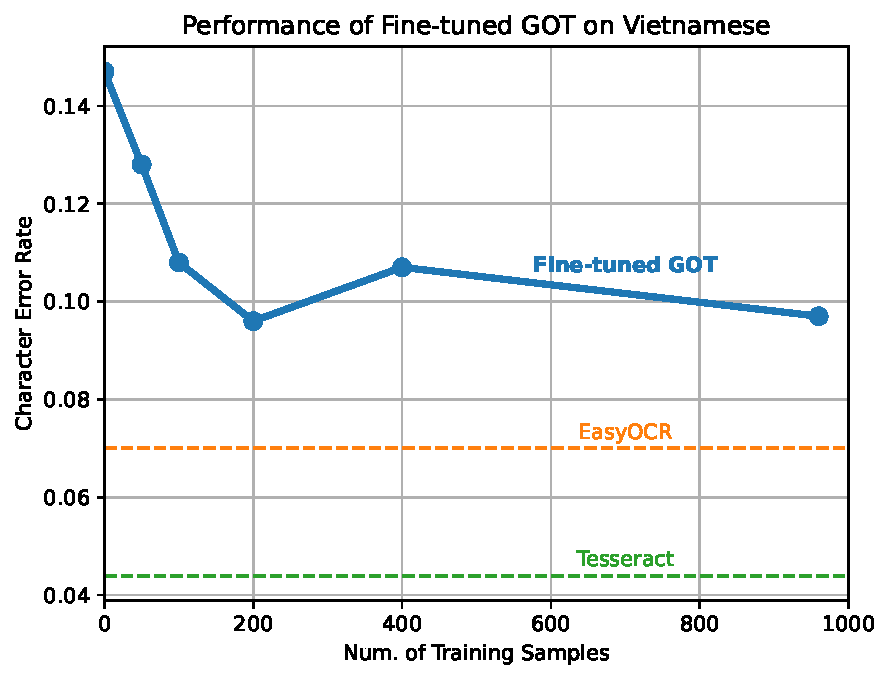
\includegraphics[width=0.8\textwidth]{images/fine-tuned-got-vietnamese.pdf}
    \caption{Performance of fine-tuned GOT on Vietnamese}
    \label{figure:fine-tuned-got-vietnamese}
\end{figure}

Figure \ref{figure:fine-tuned-got-vietnamese} presents the performance of the fine-tuned GOT models on Vietnamese (Experiment 3). 
Each GOT model was fine-tuned on different numbers of training images, and their CERs on the test dataset are plotted.
For comparison, the performance of EasyOCR and Tesseract is also included.
From the Vietnamese model results, we observed the following:

\begin{itemize}
    \item \textbf{Our best fine-tuned Vietnamese GOT model achieved a CER of 0.10.}
    Using 200 training images resulted in a 33\% reduction in error rate compared to the base GOT model without fine-tuning, which achieved a CER of 0.15.
    \item \textbf{The fine-tuned Vietnamese model underperformed relative to EasyOCR and Tesseract.} EasyOCR achieved a CER of 0.07, and Tesseract achieved a CER of 0.04.
    \item \textbf{Model performance did not consistently improve with more training data.} 
    Instead, we observed a non-monotonic trend, peaking at 200 training samples and plateauing thereafter.

    This behavior may be due to the strong pre-training of the base GOT model on English.
    Since Vietnamese uses Latin scripts with diacritics, many characters and visual patterns are shared with English.
    The base model likely already encodes strong representations for Latin characters, enabling it to adapt to Vietnamese with relatively little fine-tuning data.
    As a result, most of the learning occurs early on, and additional training data provides diminishing returns once the model has sufficiently generalized to the task.
\end{itemize}

\begin{figure}[ht]
    \centering
    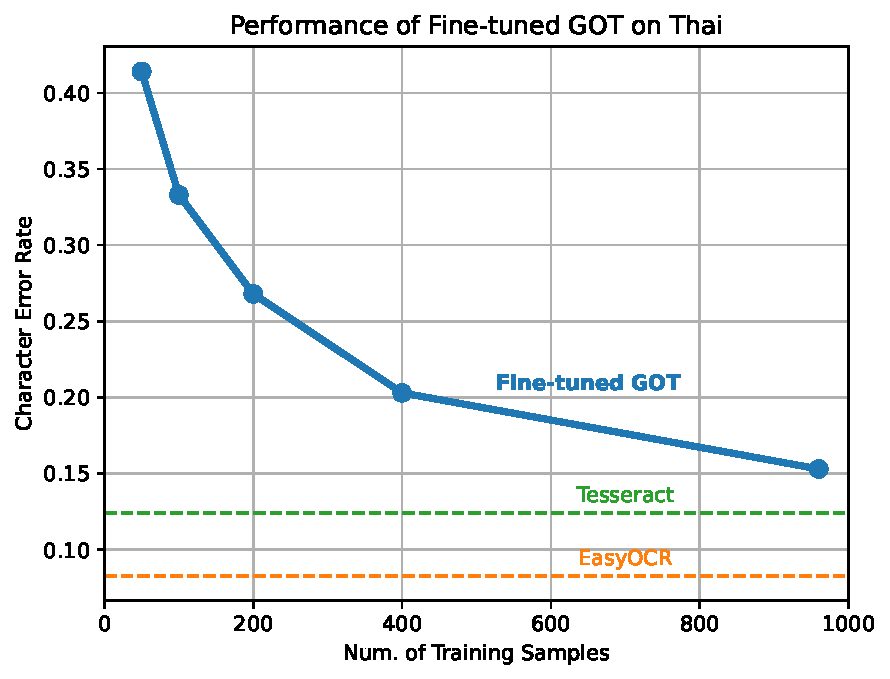
\includegraphics[width=0.8\textwidth]{images/fine-tuned-got-thai.pdf}
    \caption{Performance of fine-tuned GOT on Thai}
    \label{figure:fine-tuned-got-thai}
\end{figure}

Figure \ref{figure:fine-tuned-got-thai} presents the performance of the fine-tuned GOT models on Thai (Experiment 3). From the Thai model results, we observed the following:

\begin{itemize}
    \item \textbf{Our best fine-tuned Thai GOT model achieved a CER of 0.15.}
    In comparison, the base GOT model failed to recognize Thai characters, producing mostly Greek characters and yielding a CER of 0.90 on a sample image.
    \item \textbf{The fine-tuned Thai model also underperformed compared to EasyOCR and Tesseract,} which achieved CERs of 0.08 and 0.12 respectively.
    \item \textbf{Unlike the Vietnamese model, the Thai model consistently improved with more training data,} achieving its best performance when trained on all 960 training samples. While the CER improved with additional data, the reduction in CER diminished as the sample size increased: from 0.08 with 100 samples, to 0.06 with 200 samples, to 0.06 with 400 samples, and finally to 0.05 with 960 samples.
\end{itemize}

\subsection{Implications on Adapting OCR Systems to New Languages}

Our results demonstrate that fine-tuning is an effective strategy for adapting OCR systems to new languages.
Even with relatively small amounts of training data, it can significantly improve OCR performance.
This makes fine-tuning especially promising for low-resource languages, where large annotated datasets are often costly and time-consuming to obtain.
Our findings show that reasonable accuracy can be achieved with modest datasets, highlighting the practicality of this method in resource-constrained settings.

While fine-tuning was successful, our experiments were limited to fine-tuning GOT on noise-free synthetic data in Vietnamese and Thai. 
Future work could incorporate noisy data to improve model robustness in real-world scenarios.
Additionally, surpassing state-of-the-art tools like EasyOCR and Tesseract may require more sophisticated fine-tuning techniques. 
Although increasing the amount of training data improved performance for Thai, our Vietnamese results suggest that more data does not always lead to better accuracy. 
As such, further gains may come from exploring alternative models and optimizing fine-tuning strategies, including hyperparameter tuning.

\chapter{Conclusion}

In this study, we evaluated the performance of three OCR tools (EasyOCR, Tesseract, and GOT) on English, Indonesian, Vietnamese, and Thai.
We implemented a reusable pipeline for collecting textual data from Wikipedia and benchmarking OCR tools.
The source code of the pipeline is available on \href{https://github.com/jasonqiu212/ocr-benchmarking-on-sea-languages}{GitHub}.

Using this pipeline, we first examined OCR performance on real-world Wikipedia screenshots.
Our benchmark results reveal that OCR tools generally perform worse on Vietnamese and Thai texts than on Latin-script languages, supporting findings from previous work \parencite{ignat-etal-2022}.

We then investigated performance on synthetic documents with added noise.
Our findings show that EasyOCR was the most robust to noise, whereas Tesseract and GOT were more sensitive.
To better isolate script-related recognition errors, we classified errors by eight character types commonly found in the benchmarked languages.
Interestingly, the OCR tools performed well on native characters in languages with complex scripts like Vietnamese and Thai, challenging past studies that suggested Latin-based scripts yield better OCR performance in SEA.
The main source of errors came from the misclassification of characters outside the target language. 
Therefore, future work aiming to improve OCR accuracy can consider developing models that are better equipped to handle mixed-script content.

Lastly, we explored the effectiveness of fine-tuning GOT on Vietnamese and Thai.
We found that even with relatively little training data, fine-tuning significantly improved the base model, achieving CERs of 0.10 for Vietnamese and 0.15 for Thai.
These results demonstrate the potential and practicality of fine-tuning for adapting OCR systems to low-resource SEA languages.
To achieve state-of-the-art results, future research can explore alternative base models and optimized fine-tuning strategies.

\printbibliography[title={References}]

\clearpage
\appendix
\renewcommand{\chaptername}{Appendix}

\chapter{Wikipedia Dataset}

\begin{table}[ht]
    \centering
    \caption{Dataset of 100 Wikipedia articles used for benchmarking real-world Wikipedia screenshots in Experiment 1 (See Section \ref{section:experiment-1})}
    \label{table:real-world-wikipedia-dataset}
    \begin{tabular}{p{1in}p{4.8in}}
        \toprule
        \textbf{Category} & \textbf{Articles} \\
        \midrule
        People & Elizabeth II, Barack Obama, Michael Jackson, Elon Musk, Lady Gaga, Adolf Hitler, Eminem, Lionel Messi, Justin Bieber, Freddie Mercury, Kim Kardashian, Johnny Depp, Steve Jobs, Dwayne Johnson, Michael Jordan, Taylor Swift, Stephen Hawking, Kanye West, Donald Trump, Cristiano Ronaldo\\
        \midrule
        Present countries & United States, India, United Kingdom, Canada, Australia, China, Russia, Japan, Germany, France, Singapore, Israel, Pakistan, Philippines, Brazil, Italy, Netherlands, New Zealand, Ukraine, Spain\\
        \midrule
        Cities$^a$ & New York City, London, Hong Kong, Los Angeles, Dubai, Washington, D.C., Paris, Chicago, Mumbai, San Francisco, Rome, Monaco, Toronto, Tokyo, Philadelphia, Machu Picchu, Jerusalem, Amsterdam, Boston, Angelsberg\\
        \midrule
        Life & Cat, Dog, Animal, Lion, Coronavirus, Tiger, Human, Dinosaur, Elephant, Virus, Horse, Photosynthesis, Evolution, Apple, Bird, Mammal, Potato, Polar bear, Shark, Snake\\
        \midrule
        Buildings and structures$^b$ & Taj Mahal, Burj Khalifa, Statue of Liberty, Great Wall of China, Eiffel Tower, Berlin Wall, Stonehenge, Mount Rushmore, Colosseum, Auschwitz concentration camp, Great Pyramid of Giza, One World Trade Center, Empire State Building, White House, Petra, Large Hadron Collider, Hagia Sophia, Golden Gate Bridge, Panama Canal, Angkor Wat\\
        \bottomrule
        \multicolumn{2}{l}{\footnotesize $^a$ Singapore was replaced because it's already listed under present countries.}\\
        \multicolumn{2}{l}{\footnotesize $^b$ Machu Picchu was replaced becuase it's already listed under cities.}
    \end{tabular}
\end{table}

\end{document}
